%!TEX root = ./Paper.tex

\section{Case Studies Regular Gridshells}

\subsection{The sphere}
A simple test of our method is the meshing of a part of a sphere. We will compare our results with a reference mesh that we obtain from a special smooth parameterization of the sphere. Namely there is a smooth parameterisation of the sphere that has the property that the lengths of partial derivatives are constant throughout the surface. That means that for small discretisation steps we can produce meshes with equal edge lengths from such a parameterisation. The formula for this unit sphere can be found in \cite{voss}:
\begin{eqnarray*}
	x(u,v)&=&\sn(u+v, k)\cdot \cos(k\cdot (u-v))\\
	y(u,v)&=&\sn(u+v, k)\cdot \sin(k\cdot (u-v))\\
	z(u,v)&=&\cn(u+v, k).
\end{eqnarray*}
Here $\sn$ and $\cn$ are the Jacobi elliptic functions with modulus $k$. For different $k\in ]0,1[$ we get spheres with equal edges lengths and different shapes of parameter curves (see Fig.~\ref{fig:spheres}).

\begin{figure}[b]
\centering
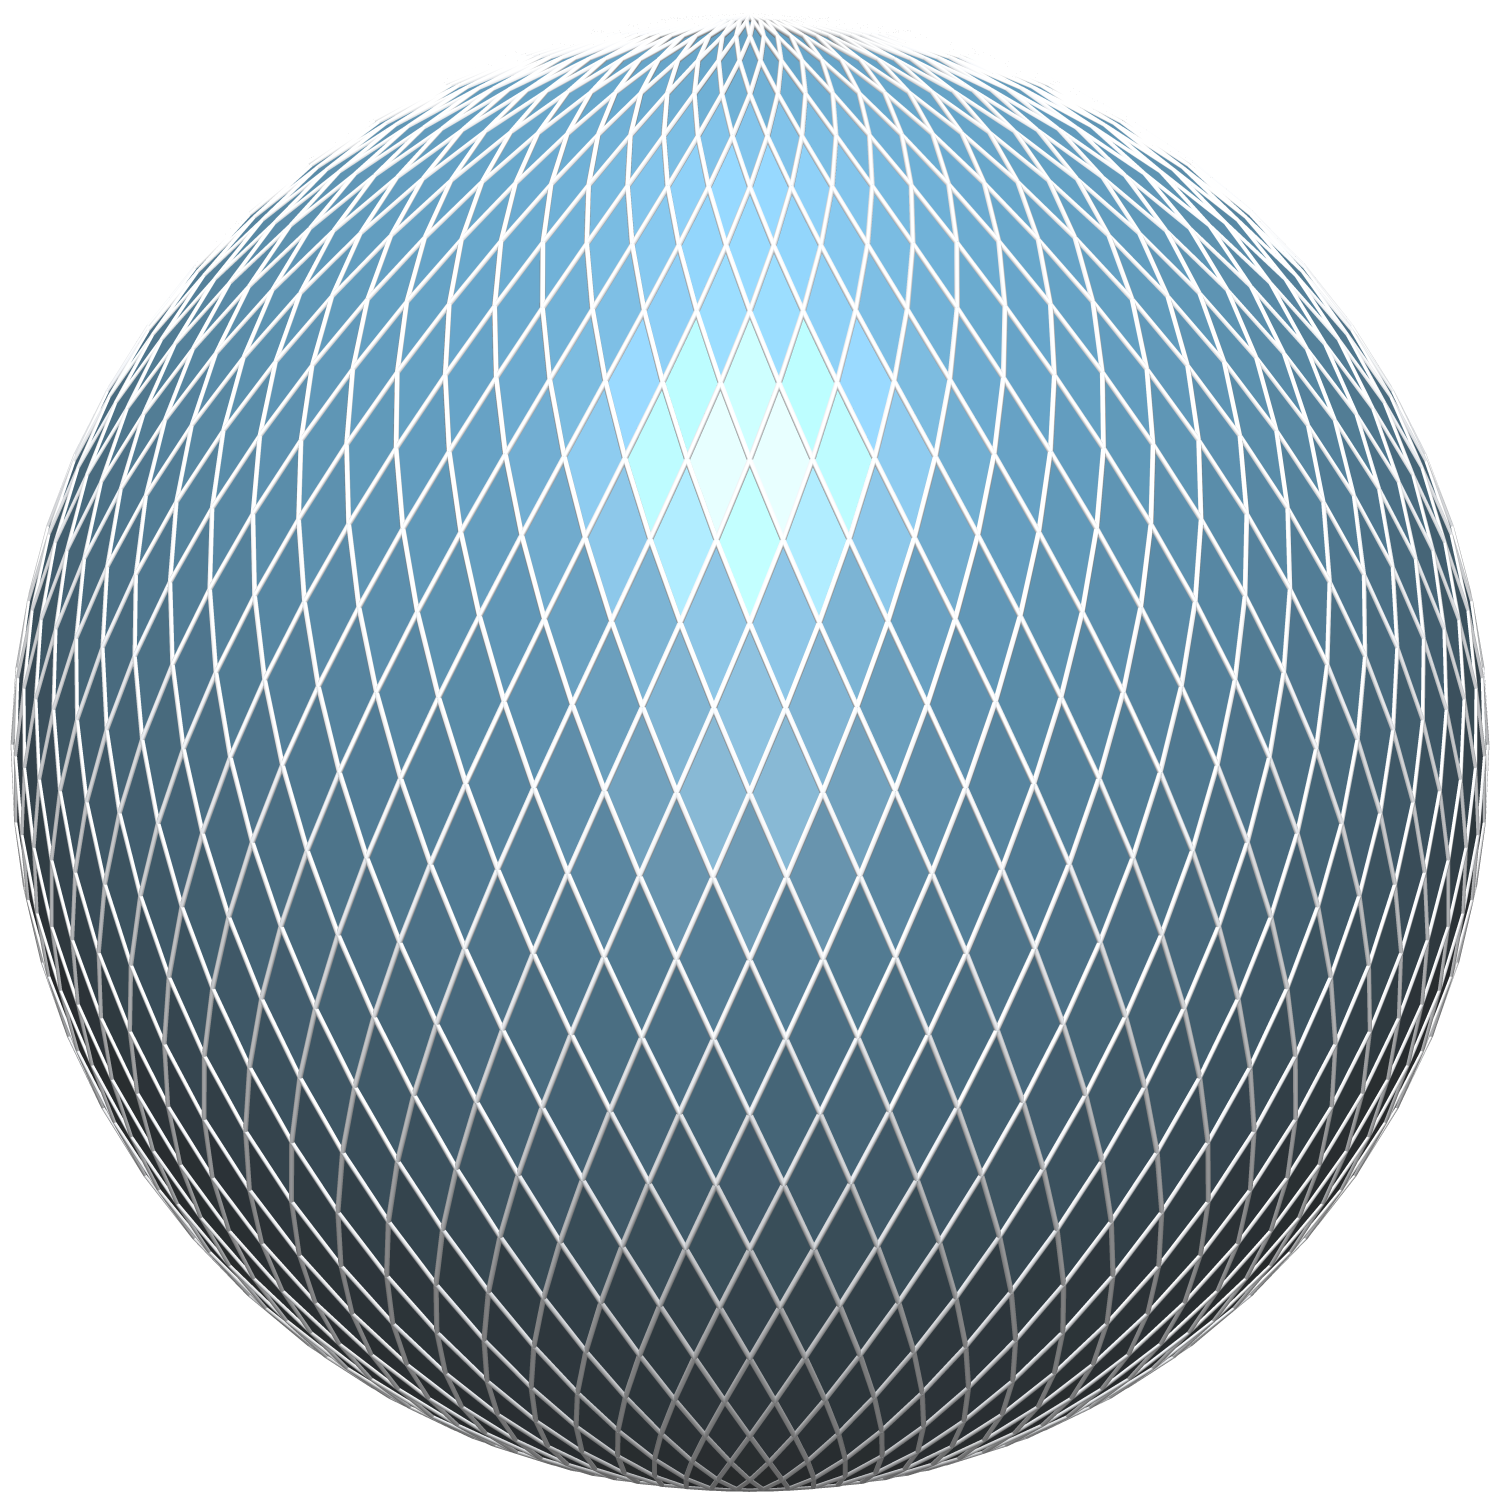
\includegraphics[width=0.32\linewidth]{images/spheres/k0_4_new.png}
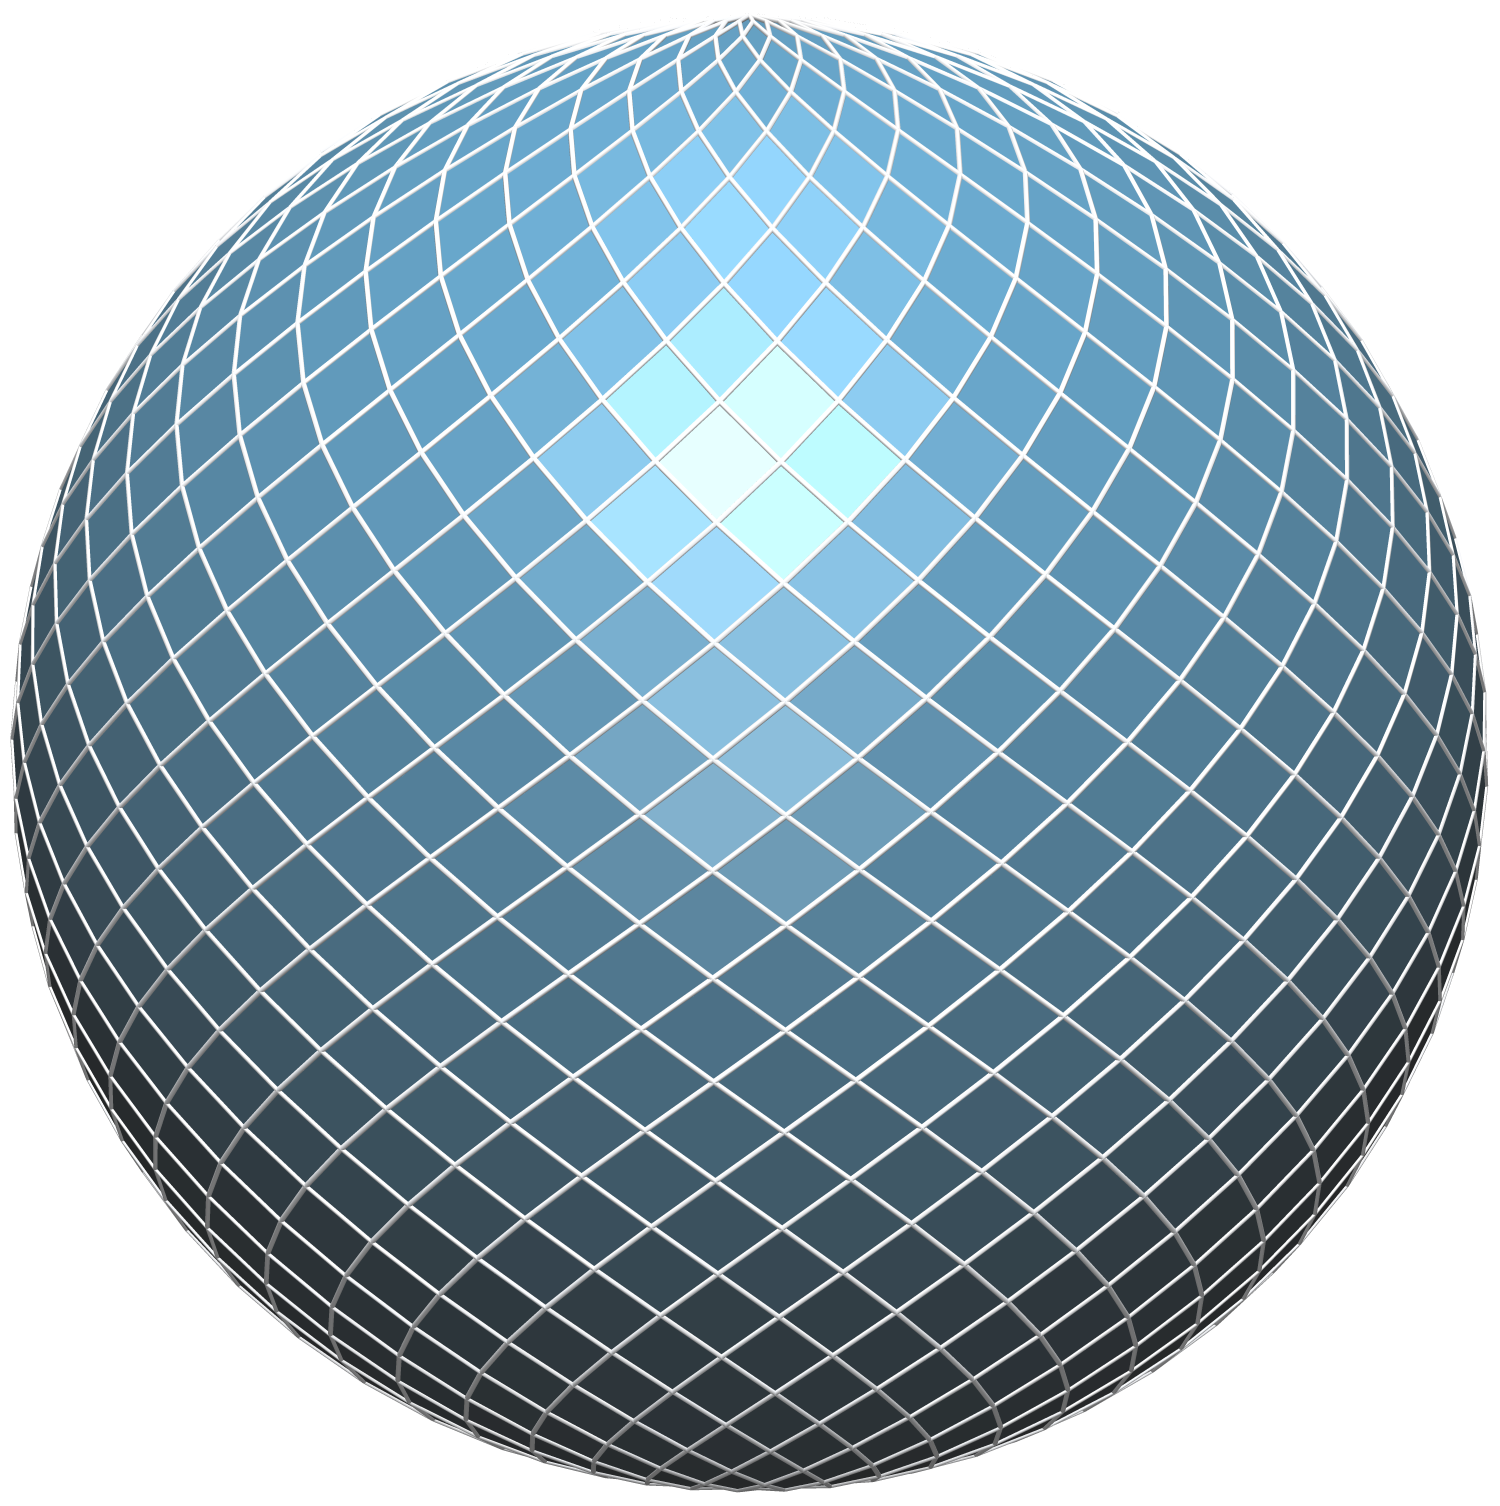
\includegraphics[width=0.32\linewidth]{images/spheres/k0_8_new.png}
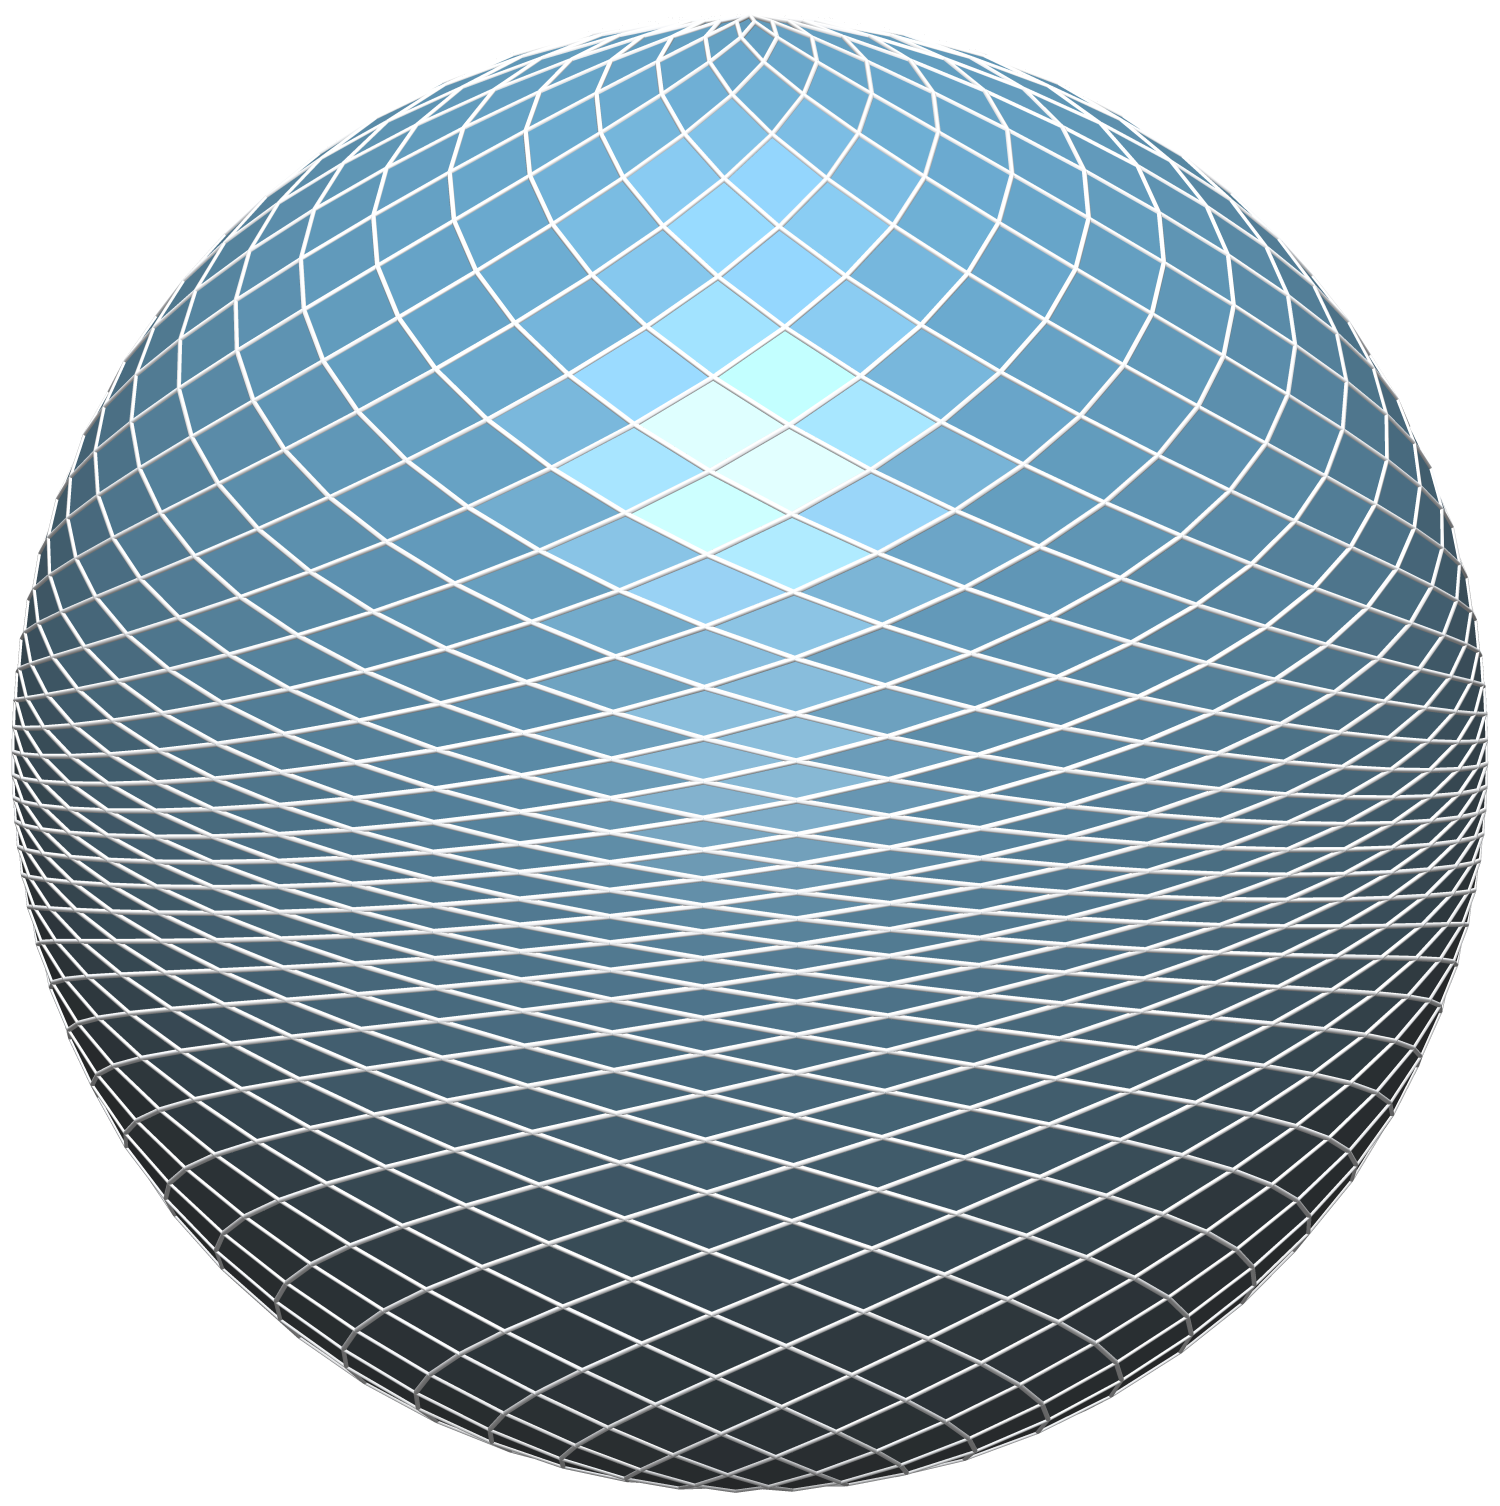
\includegraphics[width=0.32\linewidth]{images/spheres/k0_99_new.png}
\caption{Explicitly parameterised spheres with equal edges length $l=0.11$. The parameter $k$ is equal to $0.4$ (left), $0.8$ (middle), and $0.99$ (right).}
\label{fig:spheres}
\end{figure}

We measure qualitative curvature of these curves like in our energy $E_{\textrm{\scriptsize{cur}}}$ as $(\pi - \angle(e,\tilde e))^2$. Where $e$ and $\tilde e$ are opposite edges at a vertex of the quad mesh. The curvature mean of the parameter curves is decreasing for $k$ approaching zero (see Fig.~\ref{fig:curvature_plot}).
\begin{figure}[hb]
\centering
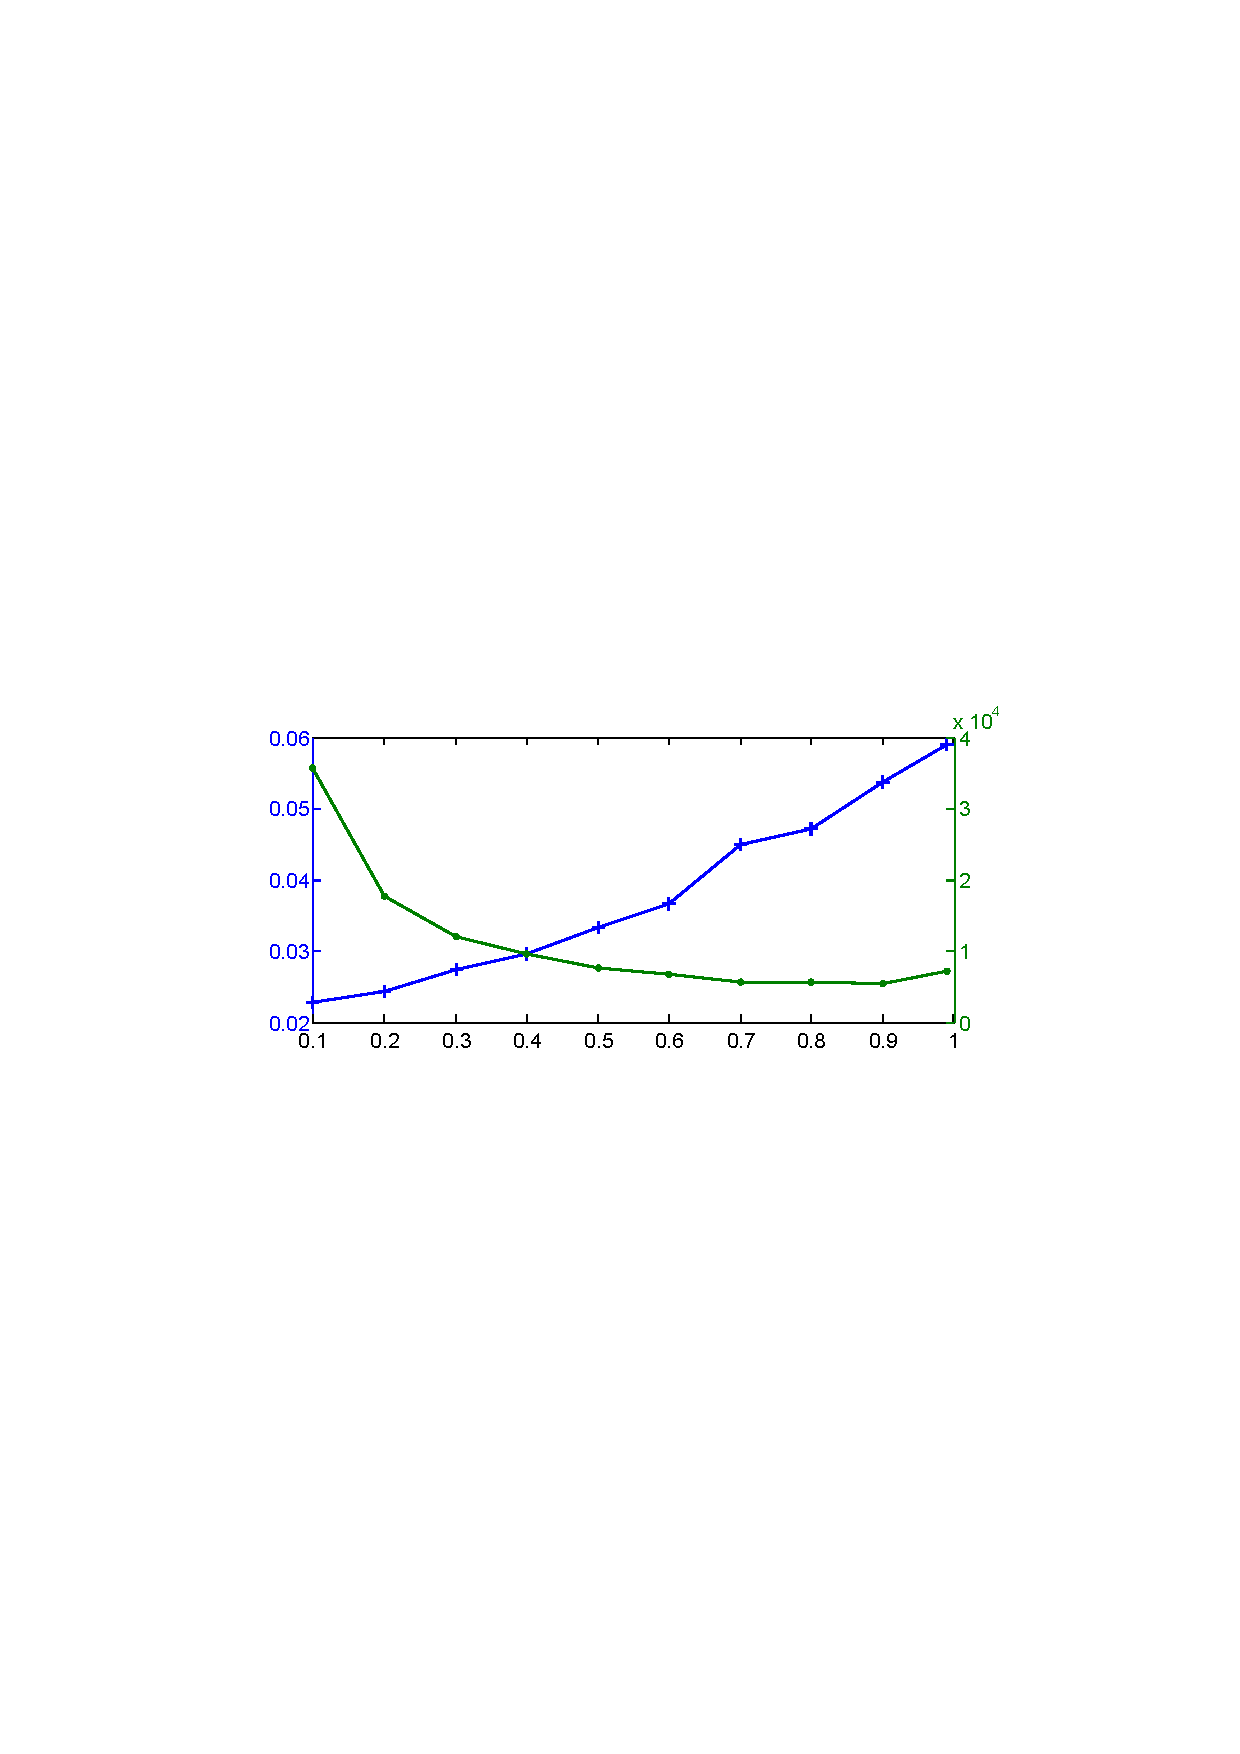
\includegraphics[width=0.7\linewidth]{images/spheres/curvature2_embedded.pdf}
\caption{The mean value of $(\pi - \angle(e,\tilde e))^2$ (blue) on parameter curves of the explicit sphere parameterization is plotted against the parameter $k$. The green curve indicates the number of edges in the corresponding mesh.}
\label{fig:curvature_plot}
\end{figure}
Using our optimisation scheme from the previous section we can reproduce the mesh shapes obtained for different $k$. The initial mesh is here a sheared conformal remesh of a part of the unit sphere (see Fig.~\ref{fig:spheres_optimised}).
\begin{figure}[ht]
\centering
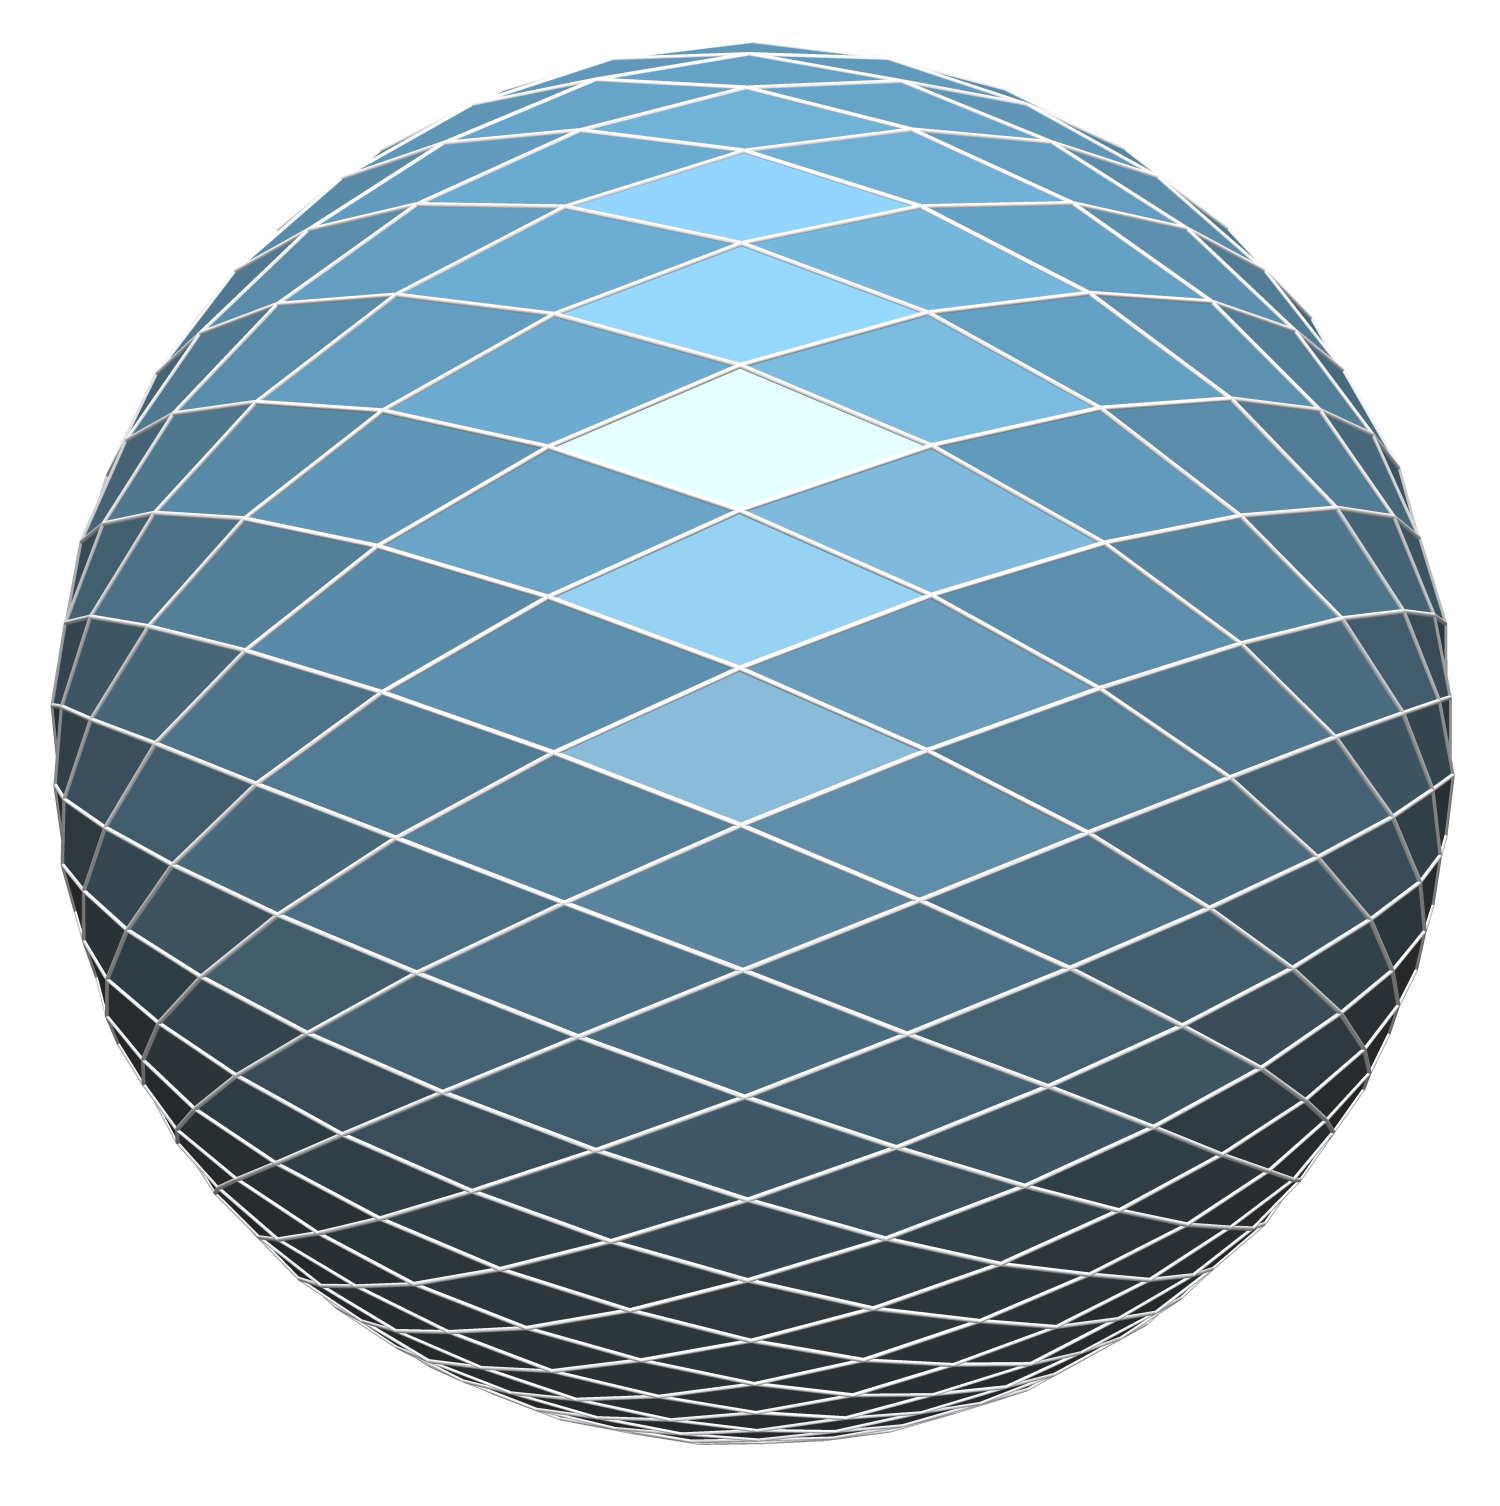
\includegraphics[width=0.32\linewidth]{images/spheres/start45_new.png}
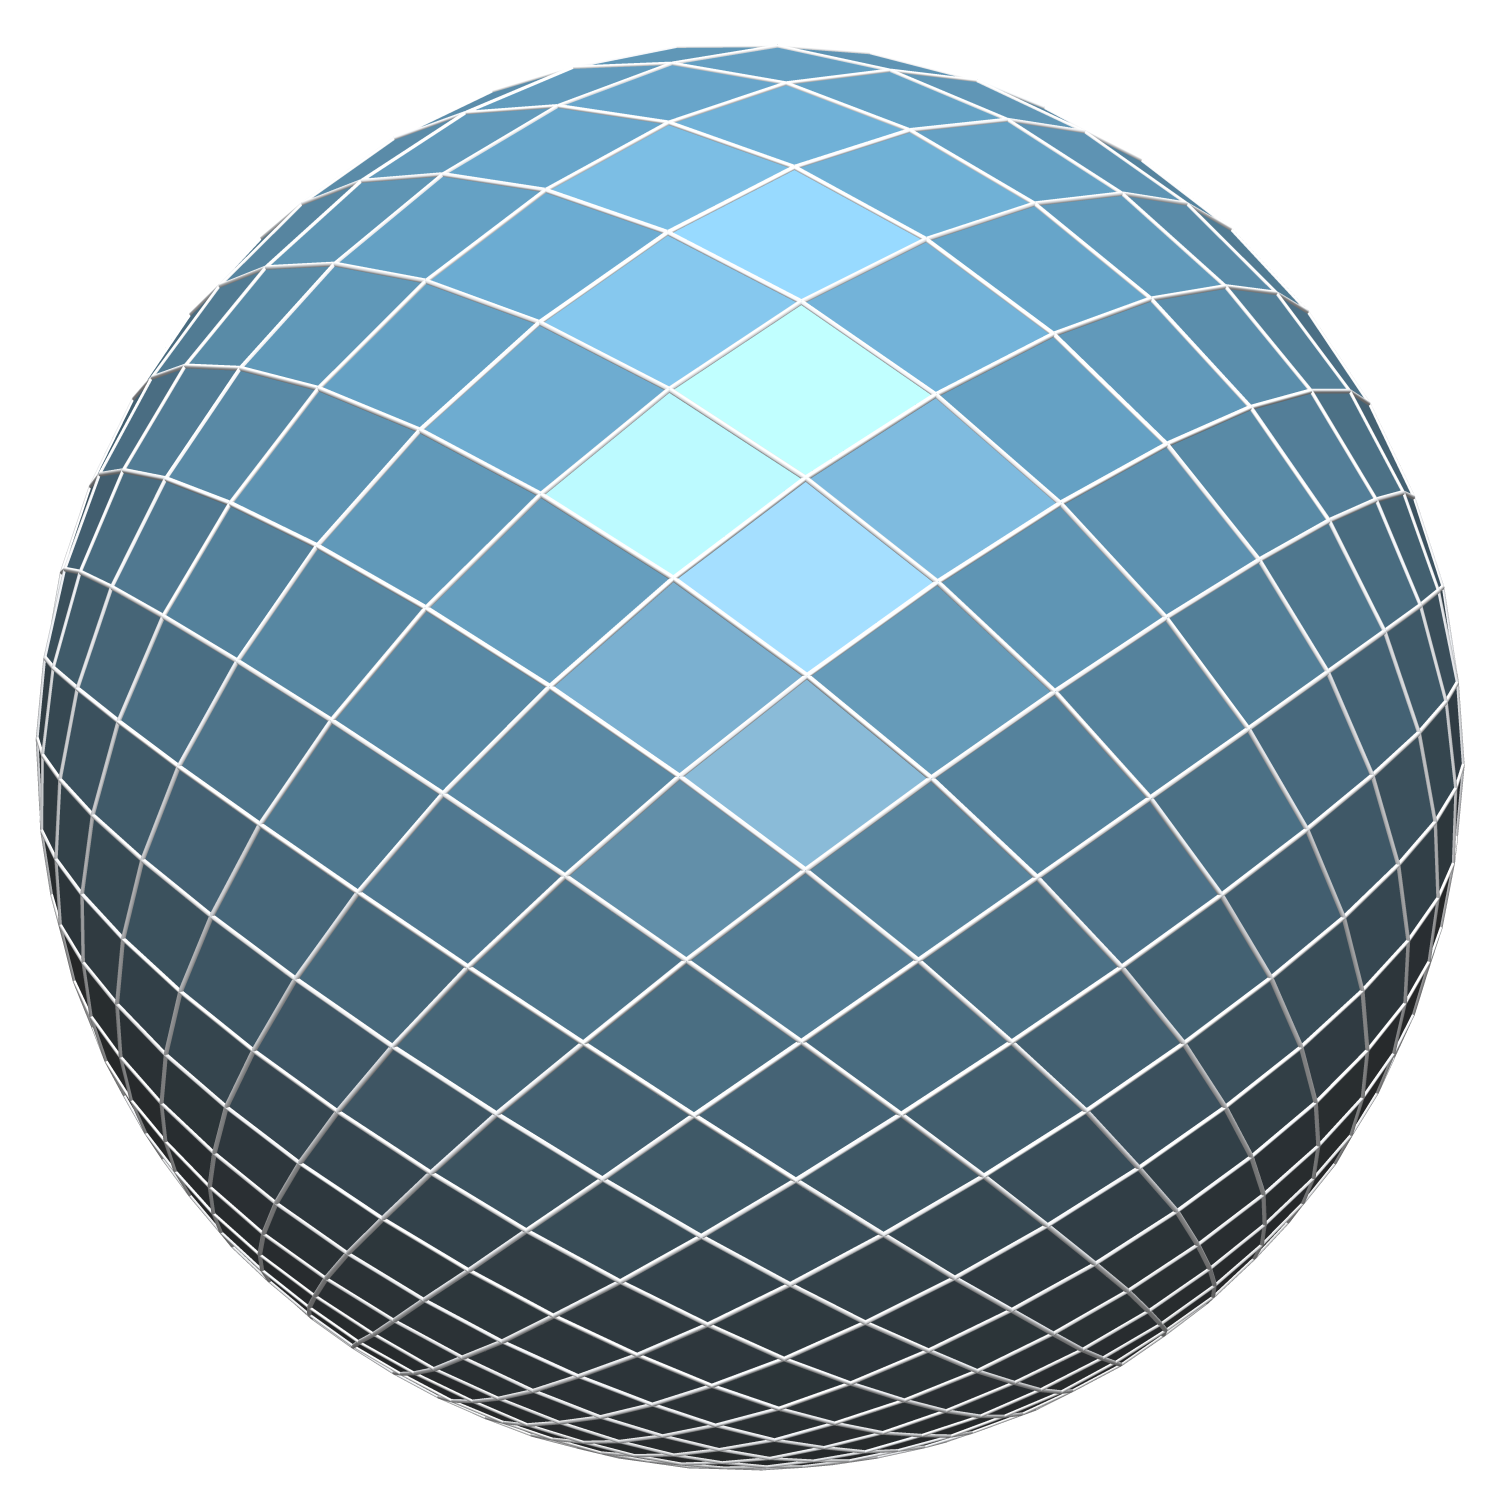
\includegraphics[width=0.32\linewidth]{images/spheres/start15_new.png}
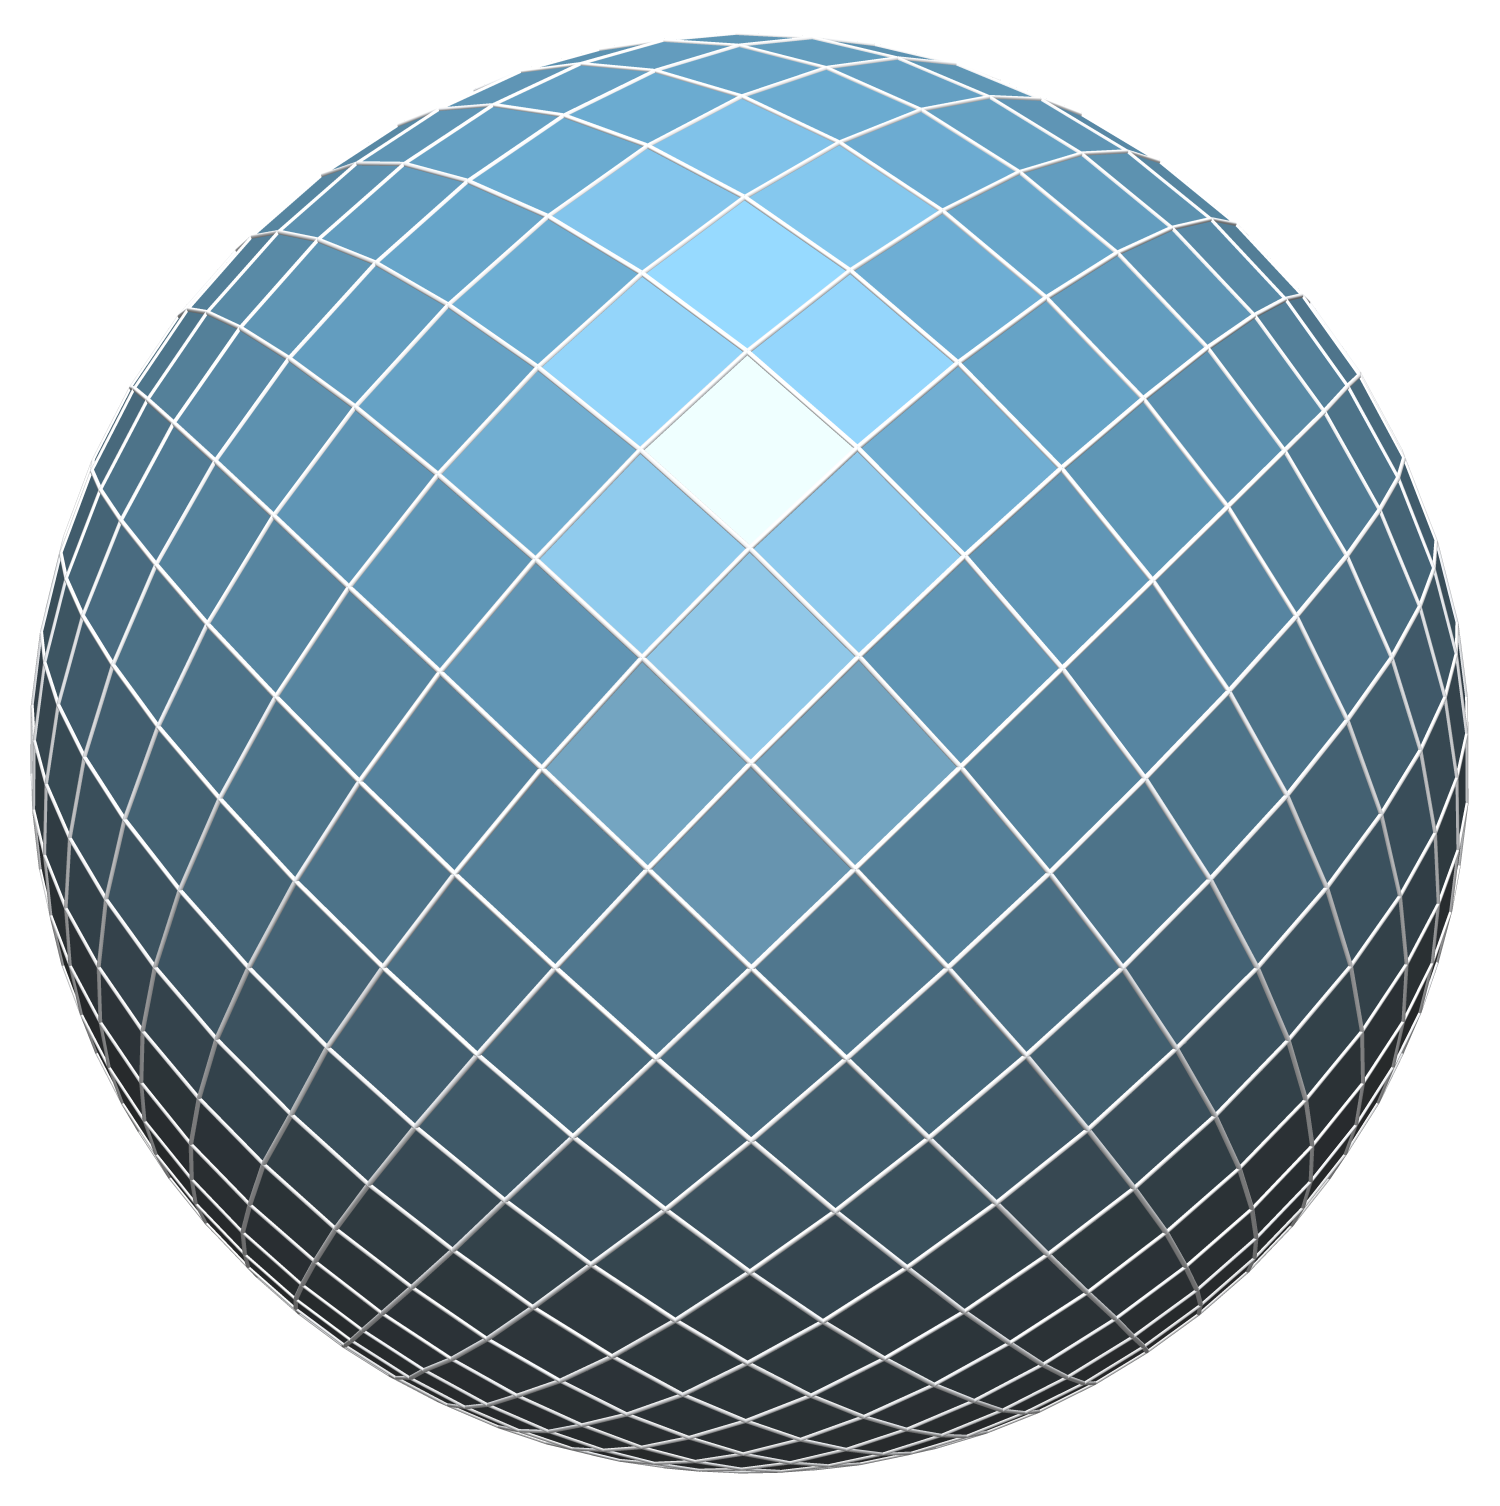
\includegraphics[width=0.32\linewidth]{images/spheres/start0_new.png}\\
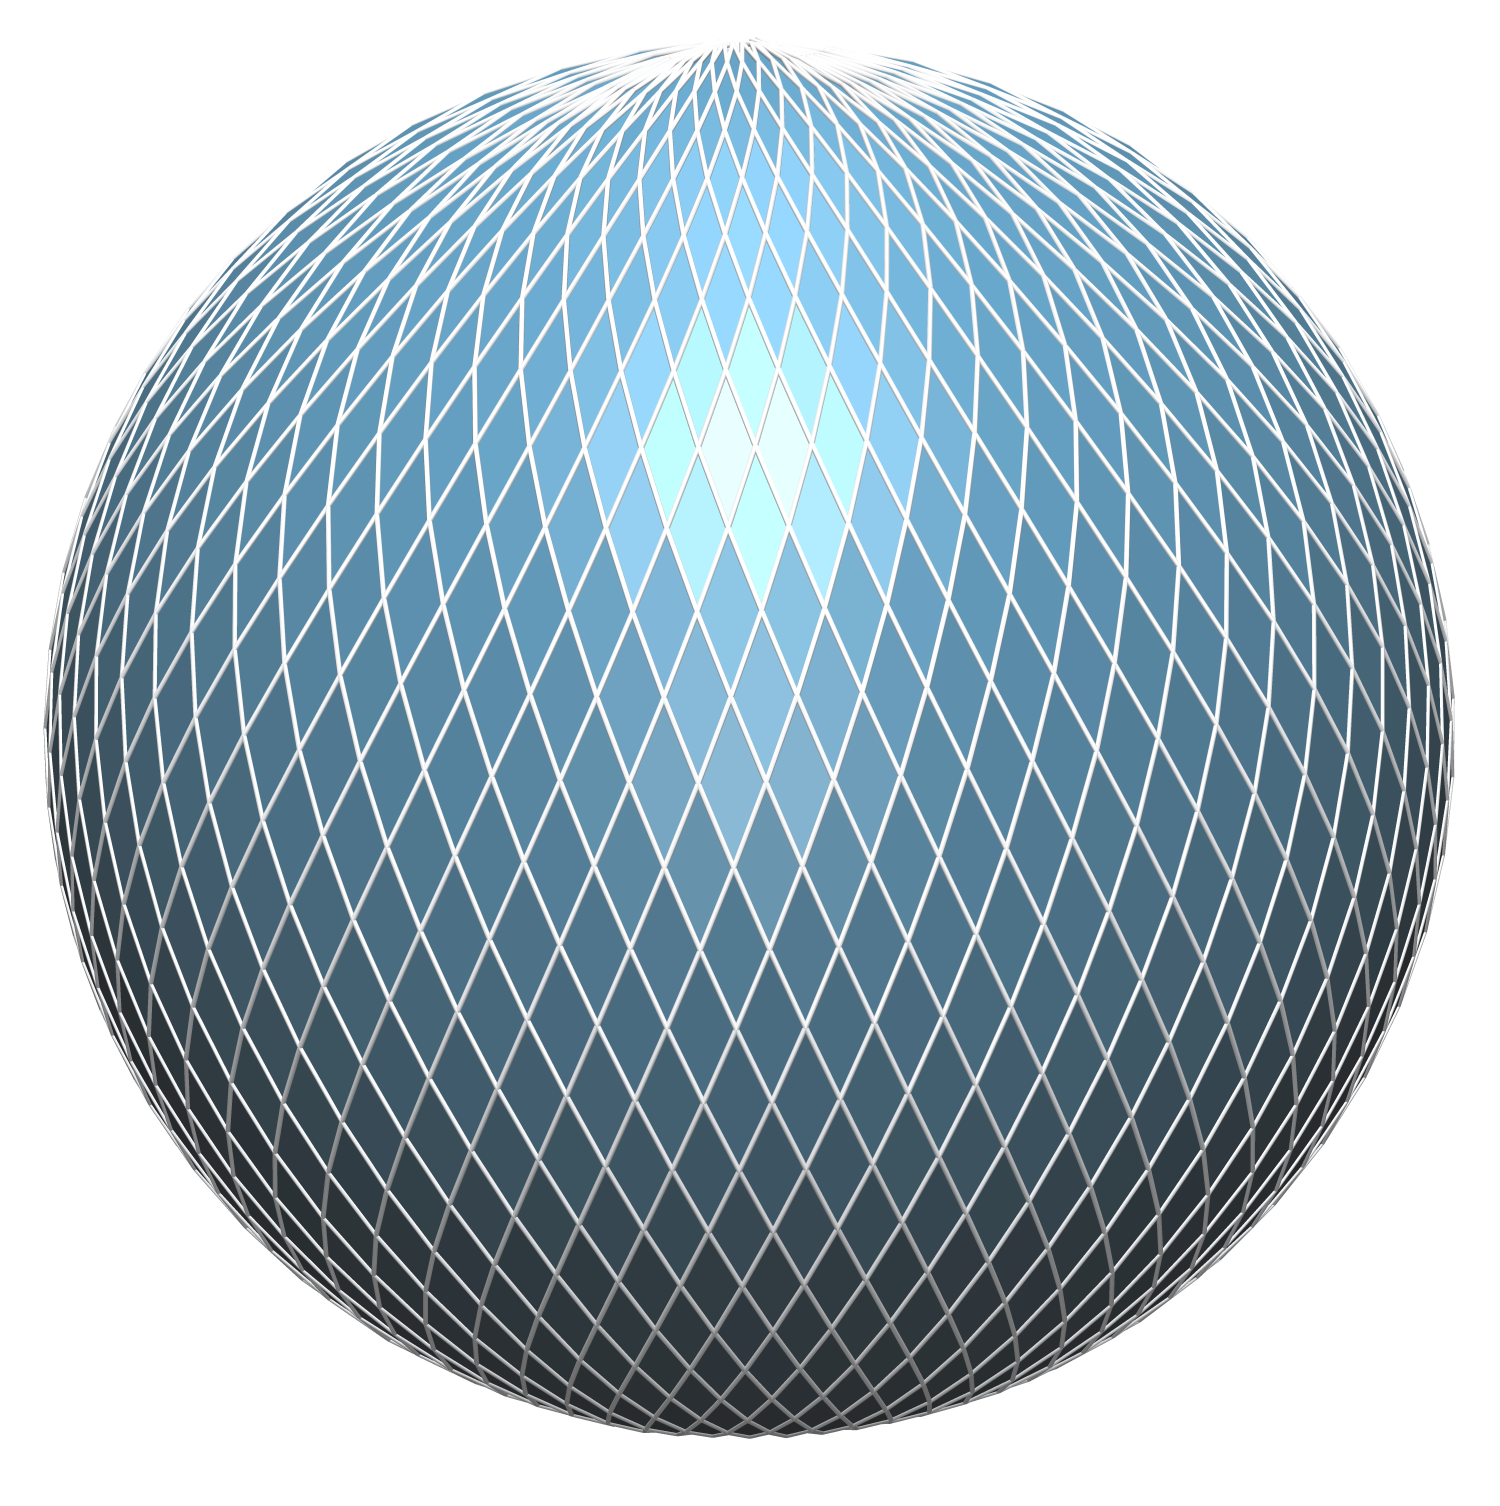
\includegraphics[width=0.32\linewidth]{images/spheres/start45_optimized_new.png}
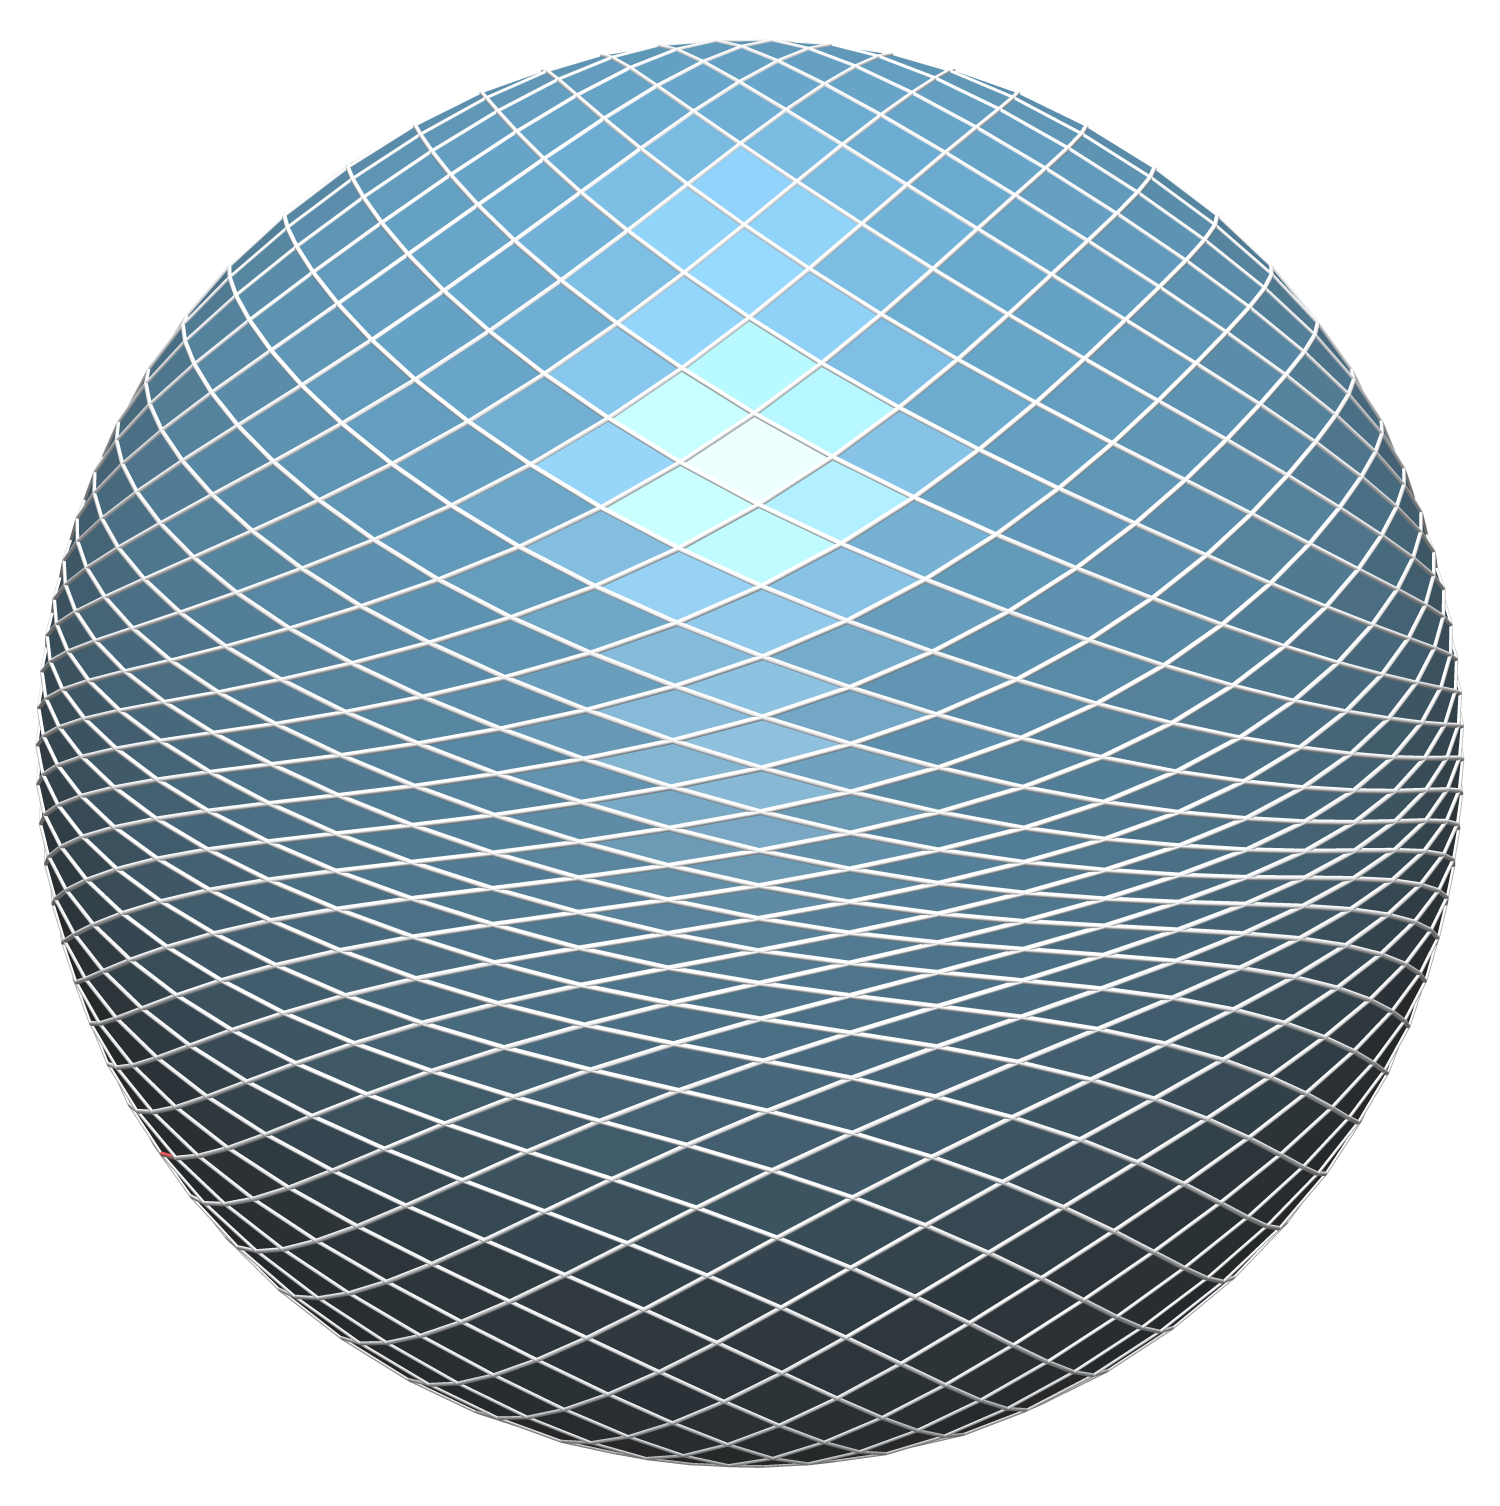
\includegraphics[width=0.32\linewidth]{images/spheres/start15_optimized_new.png}
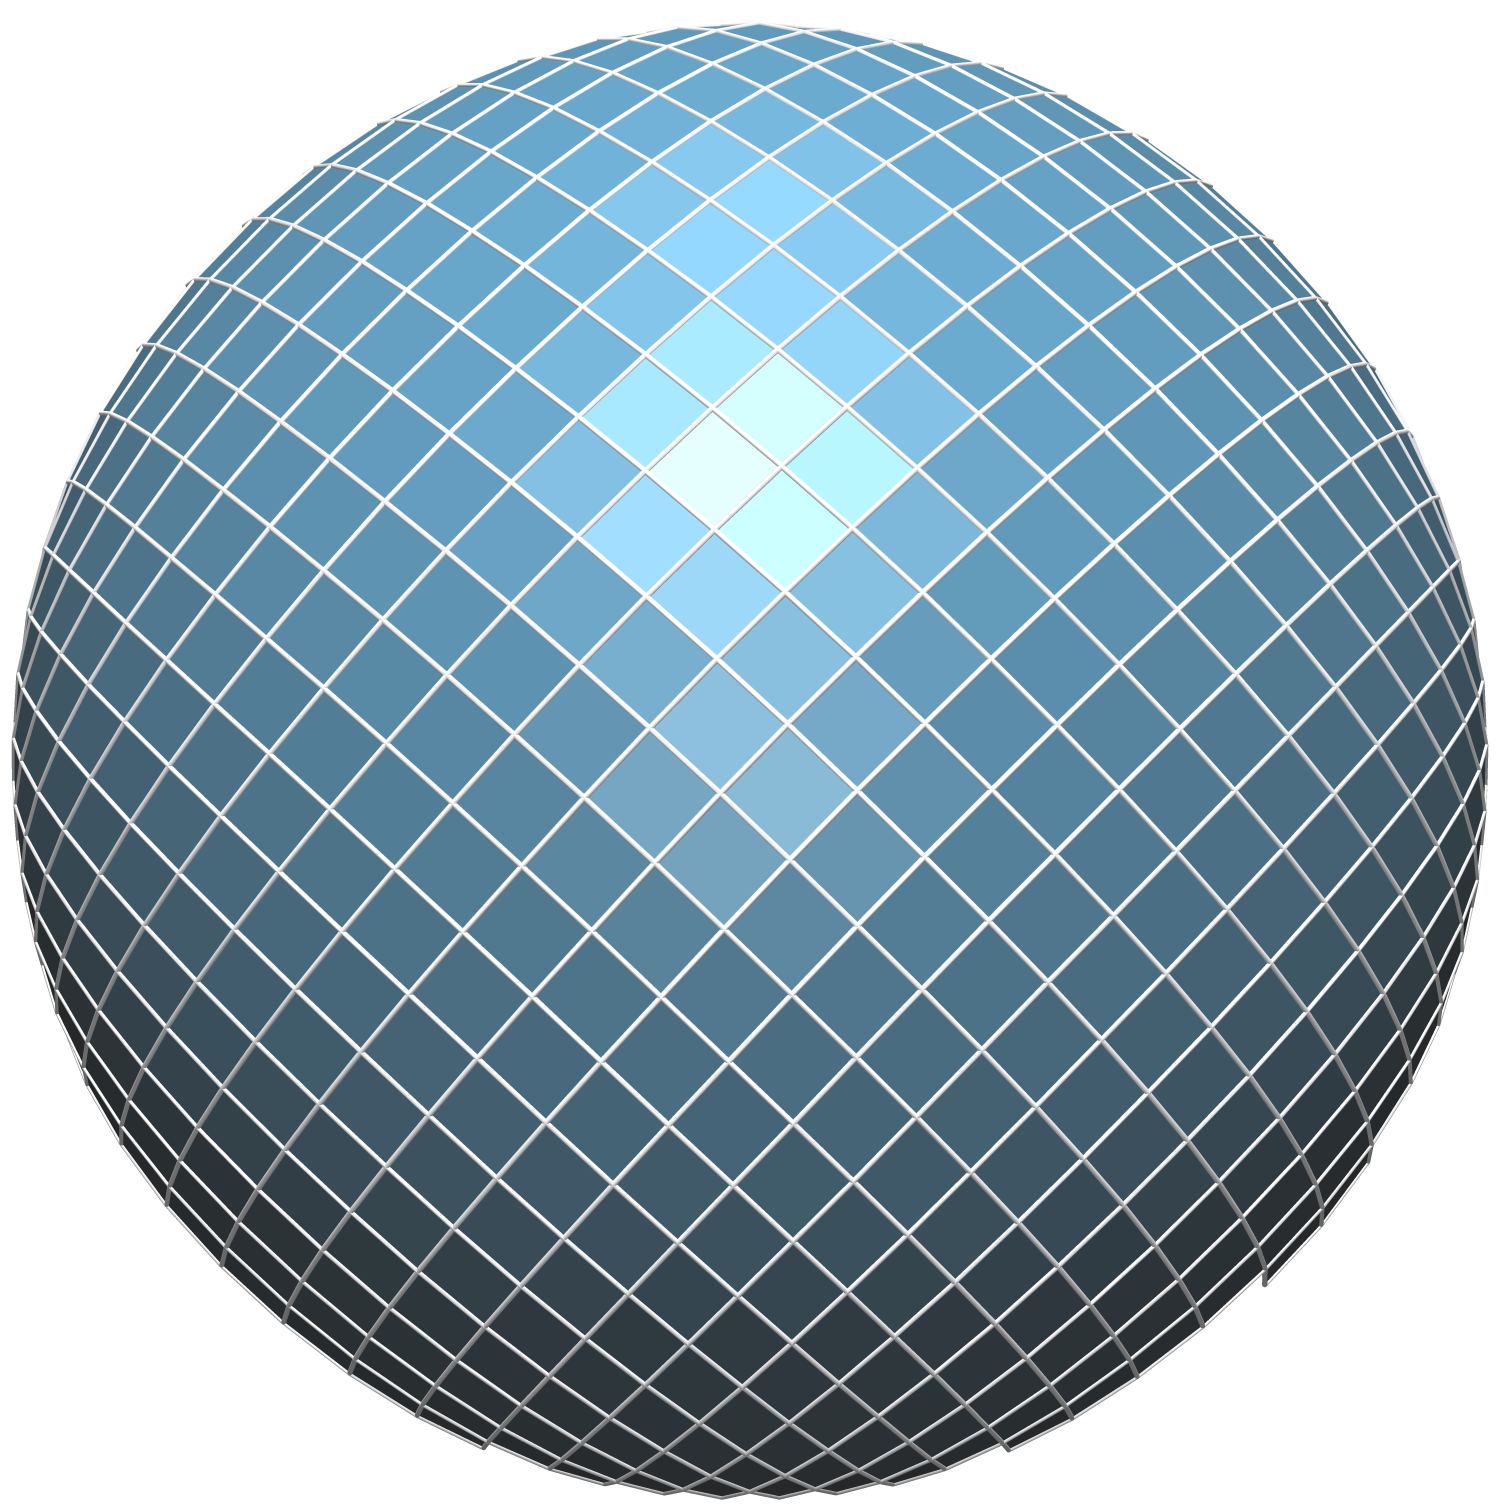
\includegraphics[width=0.32\linewidth]{images/spheres/start0_optimized_new.png}
\caption{Initialisation meshes (top) and optimised geometries (bottom). The obtained geometry depends on the initial shear angle and on the boundary shape of the mesh. This leads to geometries that correspond visually to $k\approx 0.4$ (Fig.~\ref{fig:spheres} left), $k\approx 0.9$ (Fig.~\ref{fig:spheres} middle). For an orthogonal init mesh we obtain a solution that is not contained in the family of smooth parameterizations of \cite{voss}. The edge lengths are constant and equal to $0.11$ in all solutions.}
\label{fig:spheres_optimised}
\end{figure}
As the sphere suggests there might be solutions with low curvature in the parameter curves that are not of use. In our case two angles of the quadrilaterals tend to zero with decreasing curvature. At the same time the number of edges needed for the mesh is increasing. The shear angle of the start mesh gives the family of parameterisations for the sphere and one can easily obtain a good trade-off between number of edges and curvature of the parameter curves.


\subsection{Comparison with the compass method}
Three double-curved gridshells with different types of curvature (anticlastic, synclastic and a combination of both) have been analysed with the variational method and the results compared with the grid definitions obtained with the classic compass method. The anticlastic gridshell is between 5 and 7.5m high, 14 and 15m wide and 30m long. The synclastic gridshell is between 7.5 and 10m high, 14 and 15m wide and 30m long. Finally, the gridshell with anticlastic and synclastic curvatures, analogue to the Downland Museum gridshell in Sussex, Great Britain (2002), has a height between 7.35 and 9.50m, a width between 12.5 and 16m and a length of 50m. 

The mesh size of all three grids is 1m and the starting angle between crossing directions in the centre of the gridshells is $90^\circ$. In the compass method, the starting angle corresponds to the angle between the initial curved axes \cite{IL1974}, and in the variational method to the angle between crossing segments. A high weighting factor of the $E_{\textrm{\scriptsize{ref}}}$ energy has been chosen so that a distance from the reference surface lower than 1/500 of the span length can be maintained.

In the following pictures the grid topologies resulting from both methods are shown and compared for the three gridshell structures. The curvatures of the profiles have been calculated as the reciprocal of the radius of the circles defined by three consecutive grid nodes. The curvature distributions, calculated by the variational method in terms of $E_{\textrm{\scriptsize{cur}}}$, have been also illustrated through coloured points. The size of the points is proportional to the curvature. The maximum and minimum curvatures correspond to the red and blue colours, respectively.

On the case of the anticlastic gridshell (see Fig.~\ref{fig:Compass_Anti}), the main difference between the grid topologies is located on the corners of the lateral edges. There, the topology resulting from the variational method tends to go more transversally to the front sides. Also there, the critical curvature of the grid given by the compass method is to be found. The variational method provided a grid topology with a more homogeneous curvature distribution and a maximum curvature value reduced to 87\%.

\begin{figure}[t]
\centering
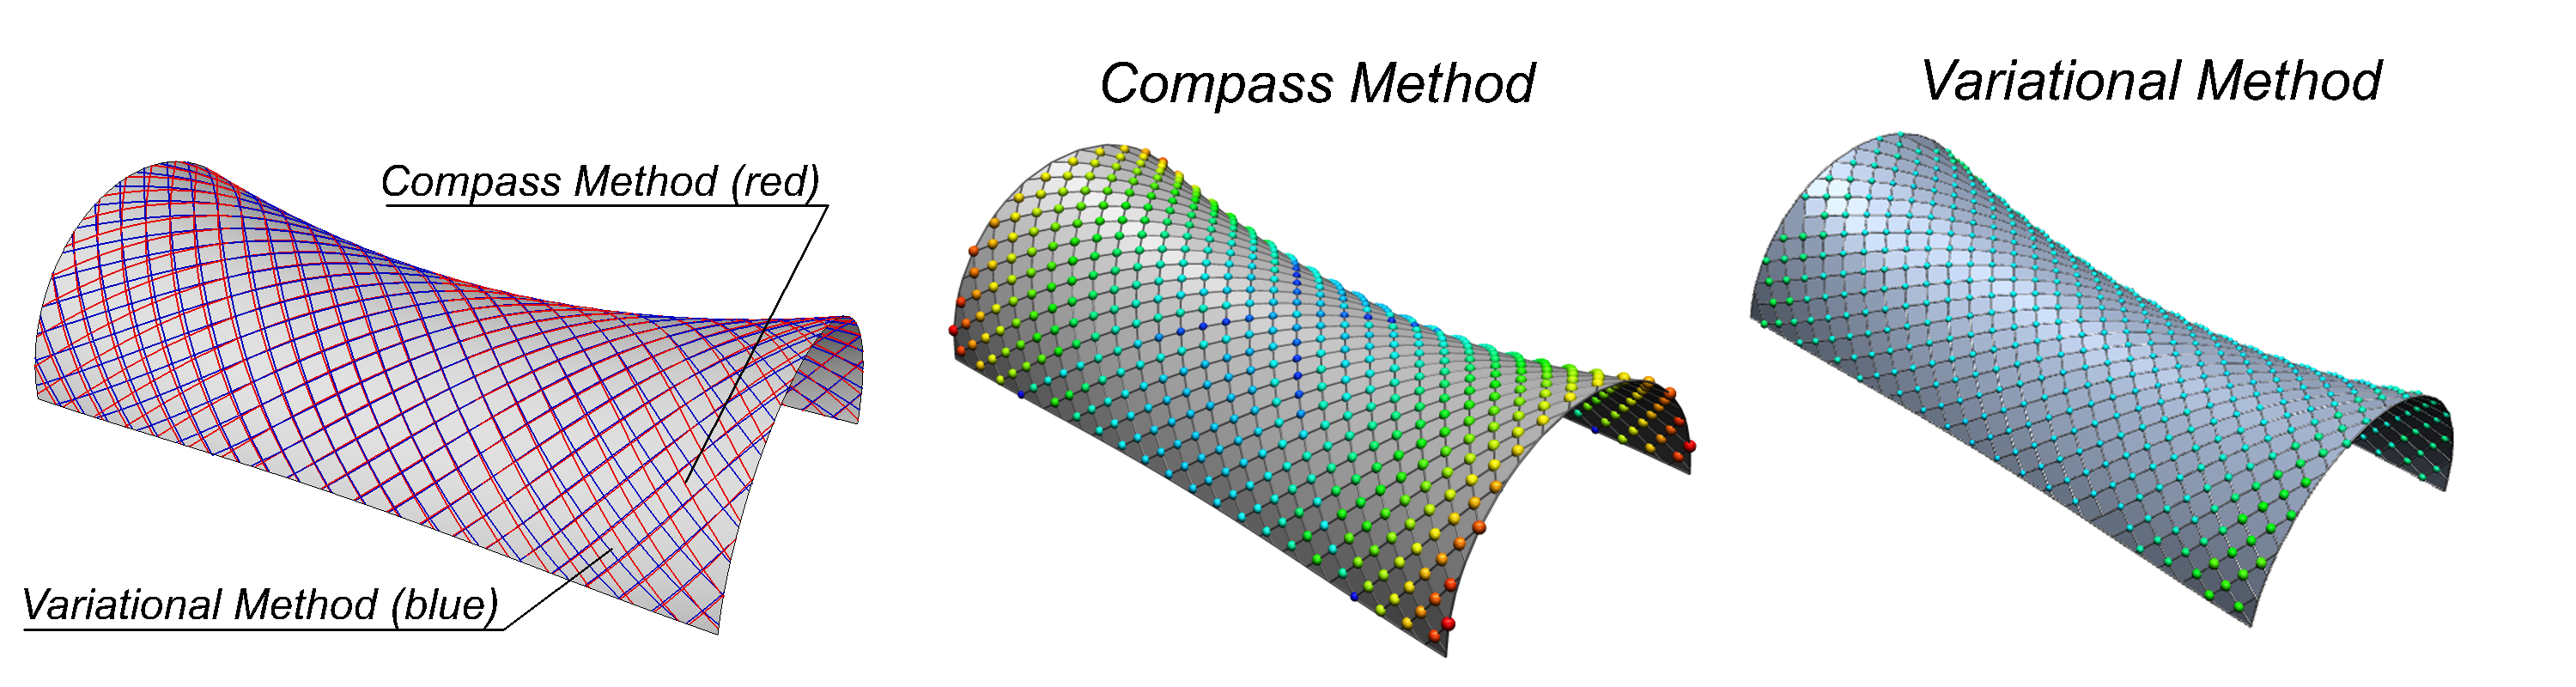
\includegraphics[width=1.0\linewidth]{images/CaseStudies_Regular/Compass_Anti.png}
\caption{Comparison between grid topologies for an anticlastic gridshell. The grid topology resulting from the compass method presents extreme curvature values (large red nodes) on the corners of the lateral edges. The configuration obtained with the variational method shows a more homogeneous curvature distribution and lower curvature values (smaller nodes).}
\label{fig:Compass_Anti}
\end{figure}

\begin{figure}[b]
\centering
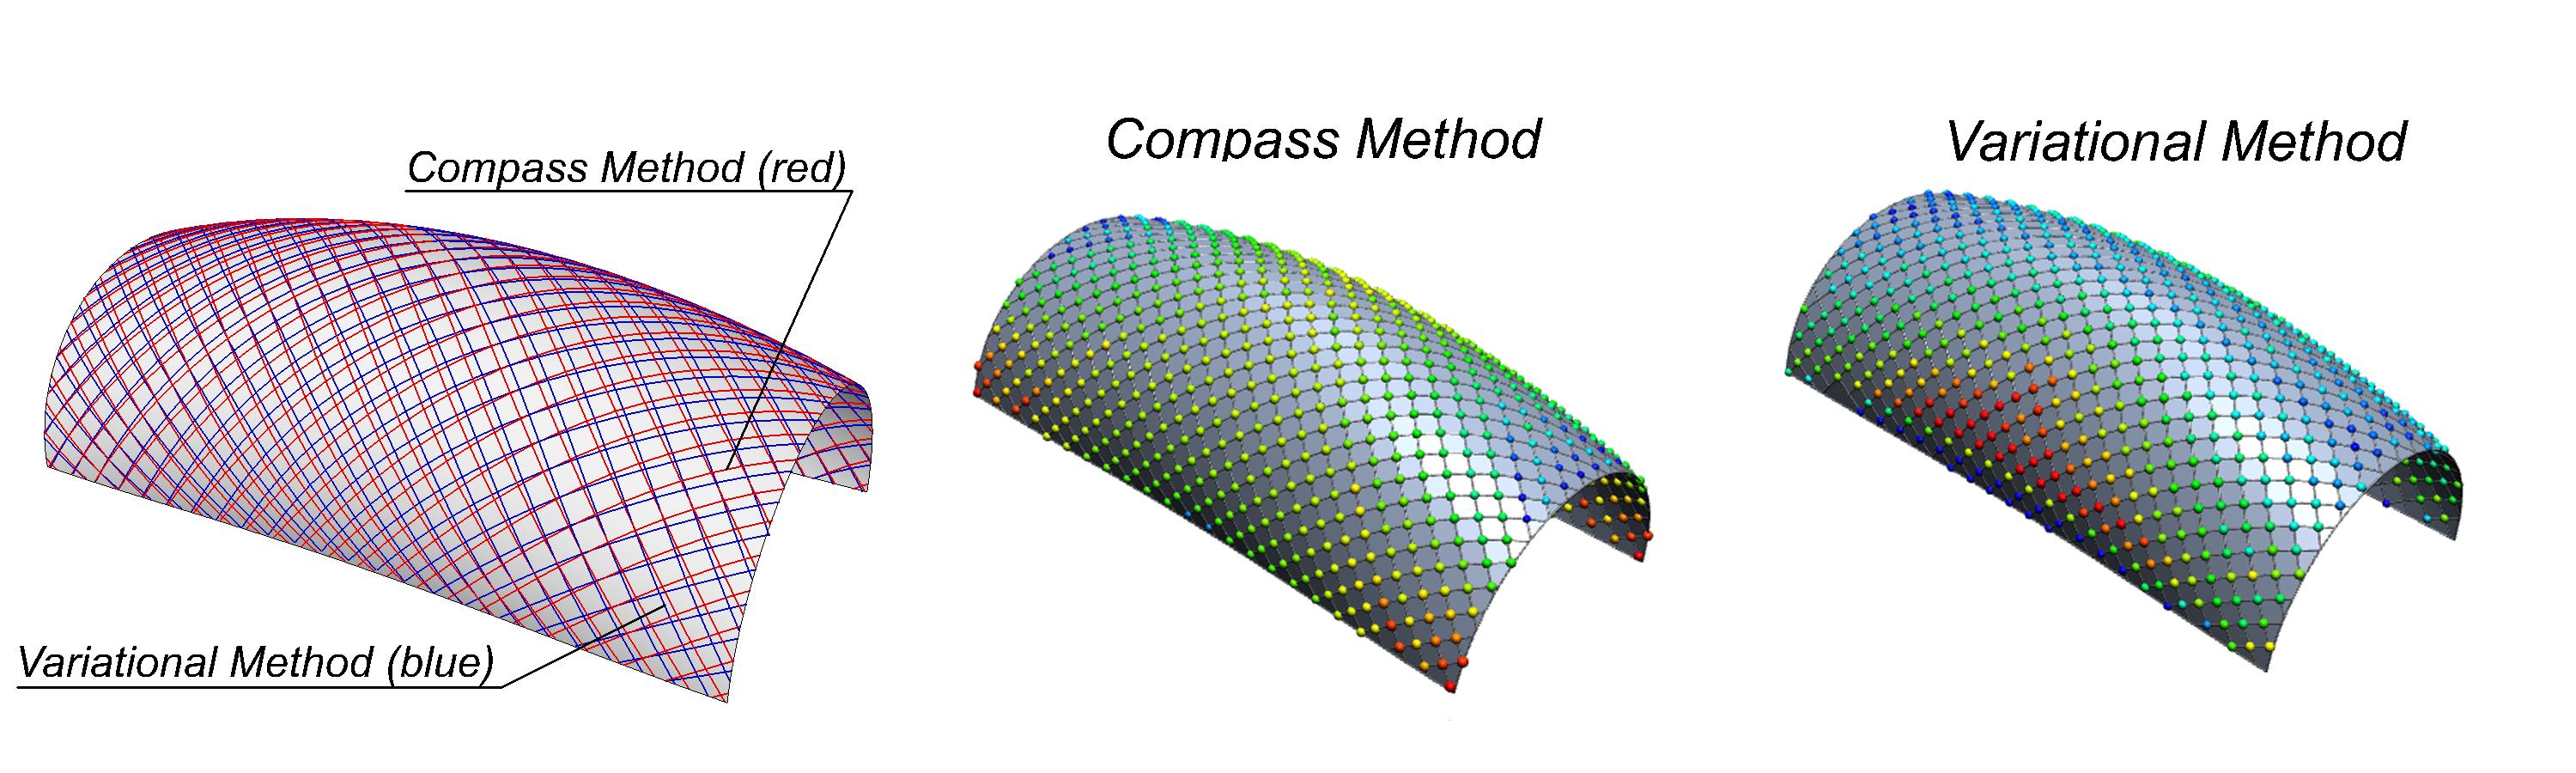
\includegraphics[width=1.0\linewidth]{images/CaseStudies_Regular/Compass_syn.png}
\caption{Comparison between grid topologies for a synclastic gridshell. The grid topology resulting from the compass method presents again extreme curvature values (large red nodes) on the corners of the lateral edges. The configuration obtained with the variational method owns lower maximum and mean curvature values.}
\label{fig:Compass_Syn}
\end{figure}

On the case of the synclastic gridshell (see Fig.~\ref{fig:Compass_Syn}), slight differences can be found on the whole lateral sides between the grid topologies obtained with both methods. The grid configuration given by the compass method presents extreme curvature values on the corners of the lateral edges and on the gridshell crown. The variational method provided a grid configuration with lower curvature values on the top and higher on the bottom of the gridshell, the  maximum profiles curvature could be reduced to 90\% compared to the compass method.

On the case of the gridshell analogue to the Downland Museum (see Fig.~\ref{fig:Compass_Downland}), differences between the grid topologies increase when approaching to the face sides. In both methods, higher curvature values are to be found on the crowns and lower on the valleys. By the grid resulting from the variational method, extrem curvature values are less concentrated as in the compass method configuration. The maximum profiles curvature could be minimized to 88\%.

\begin{figure}[ht]
\centering
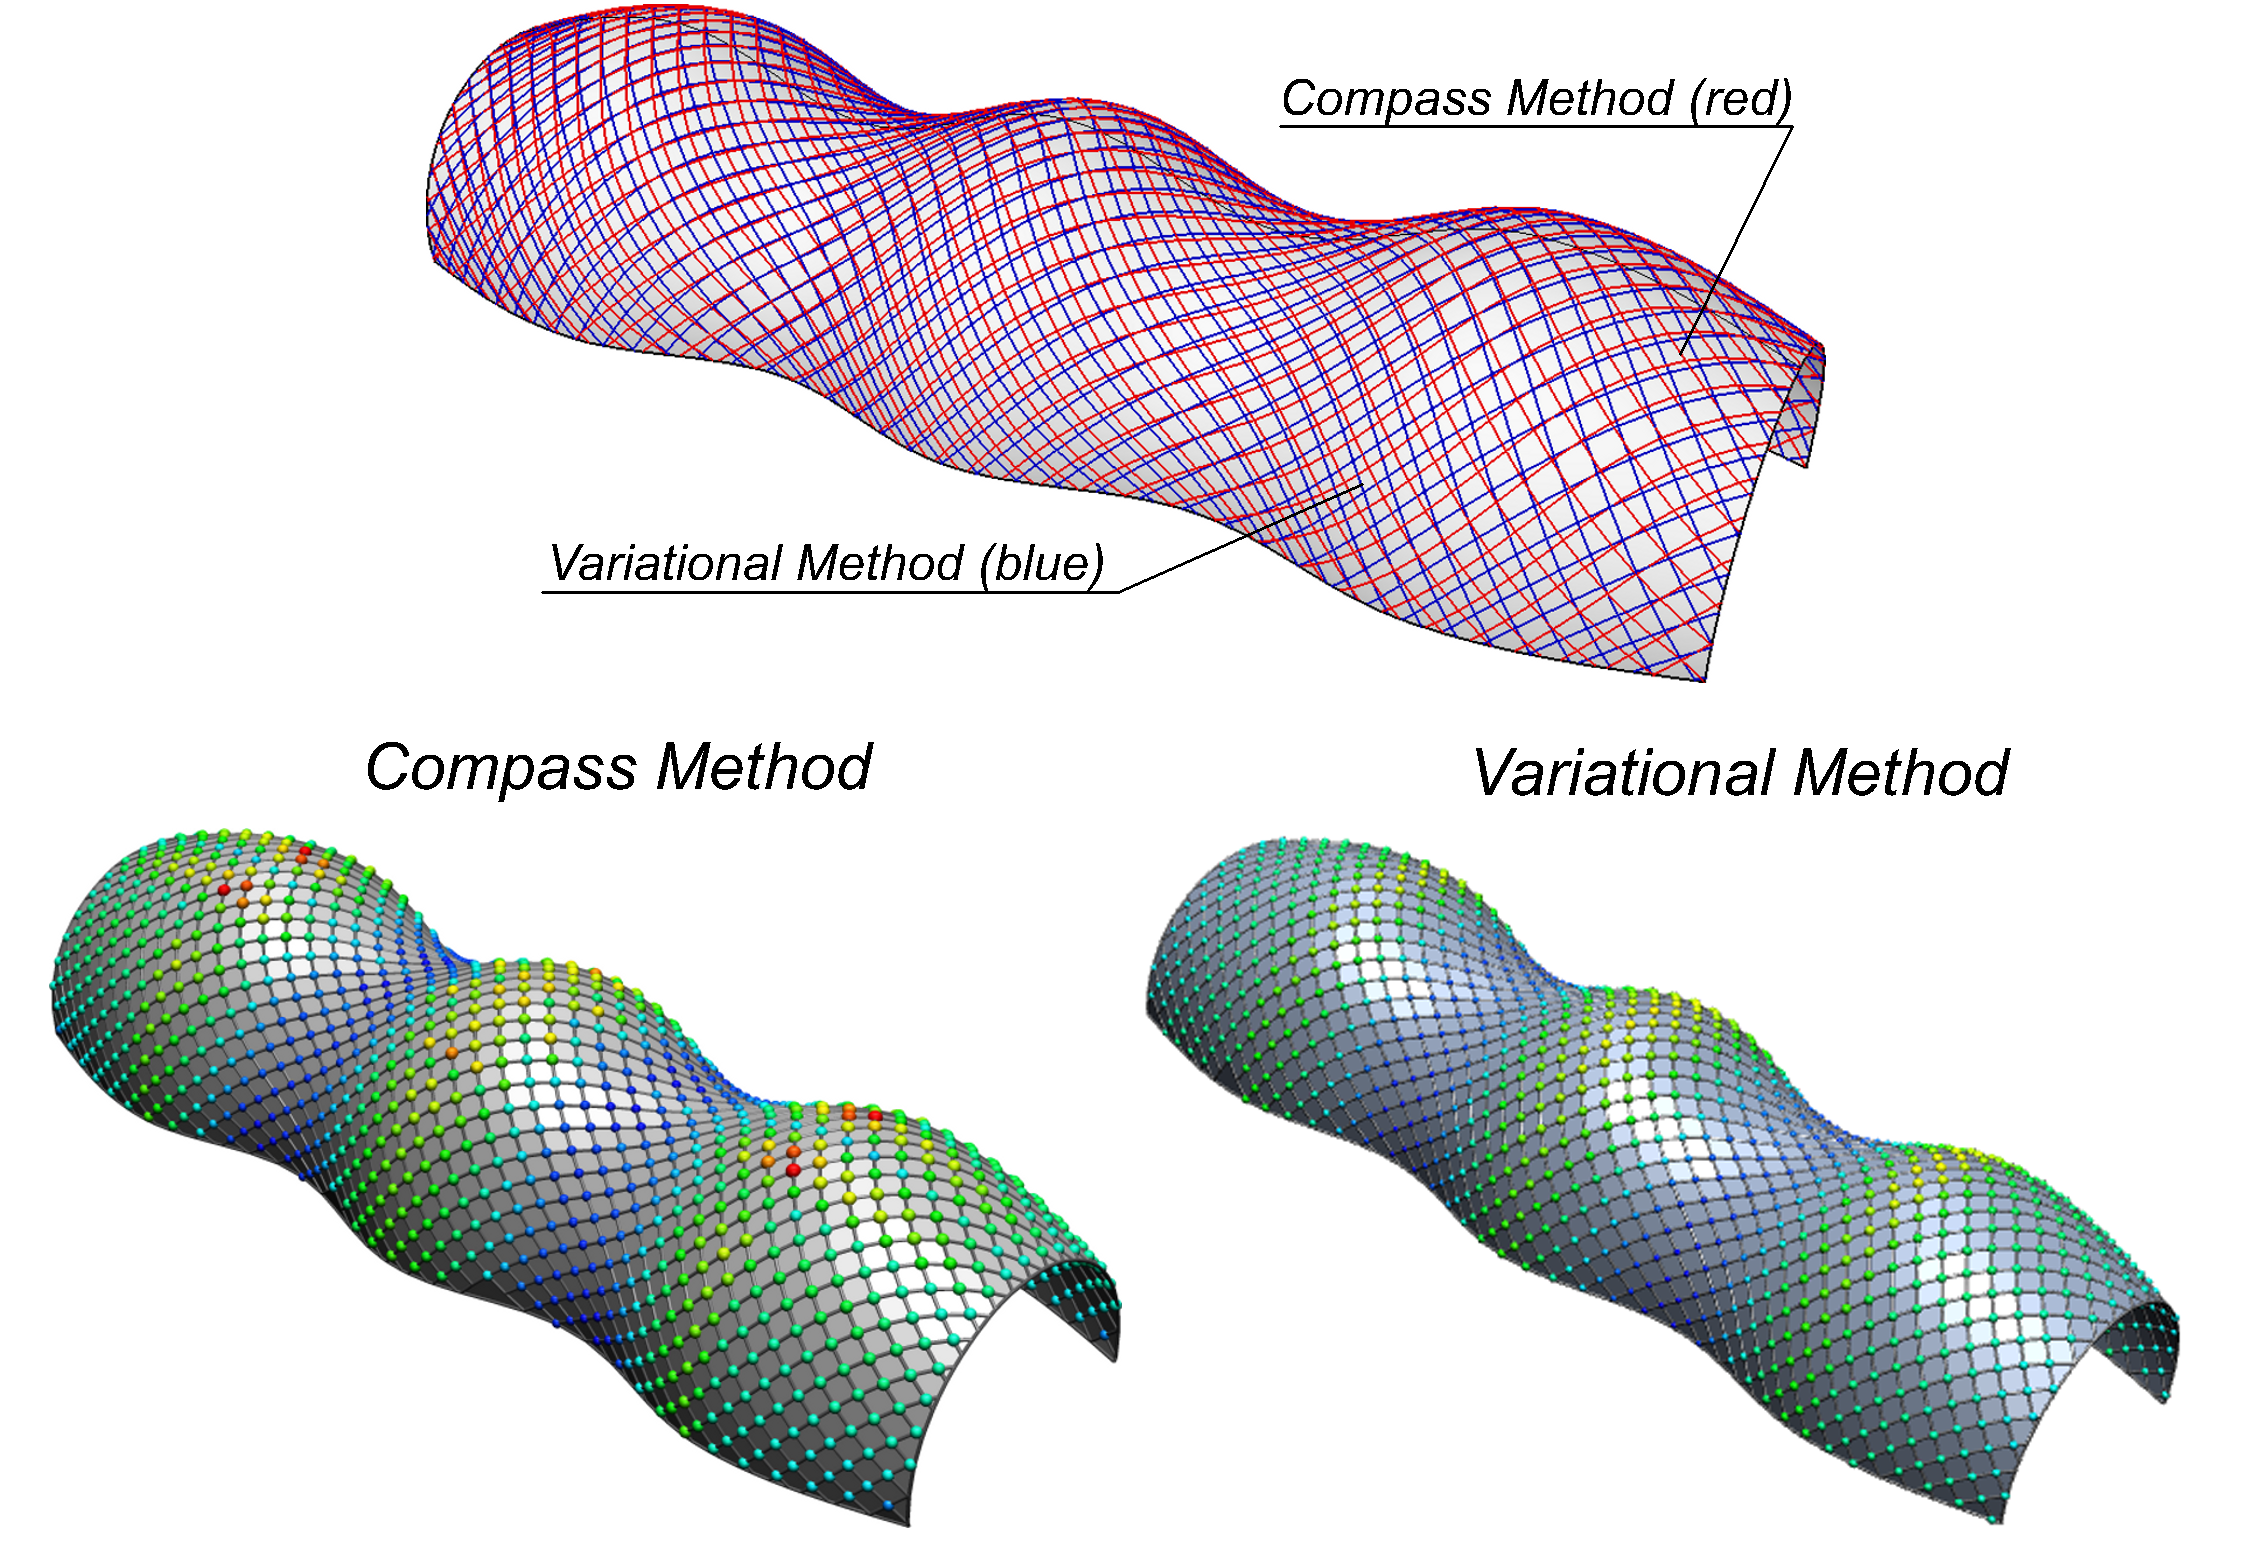
\includegraphics[width=0.80\linewidth]{images/CaseStudies_Regular/Compass_Downland.png}
\caption{Comparison between grid topologies for the Downland-like gridshell. In both methods, higher curvature values are located on the crowns (red nodes) and lower on the valleys (blue nodes). With the variational method, a higher distribution of the extreme profiles curvatures could be obtained.}
\label{fig:Compass_Downland}
\end{figure}

With the variational method, grid topologies with lower and more homogeneously distributed profiles curvatures than by the compass method could be obtained. A further optimisation could be achieved by using another starting mesh with different edge angles, by tolerating a higher distance from the reference surface or by allowing variation on the segment lengths. In the following chapters the weighting factors of the {it\ reference surface} and {it\ segments length} energies have been minimized in order to achieve a higher reduction of the grid curvature.

\subsection{Further optimisation by allowing more distance to surface reference}

\begin{figure}[t]
\centering
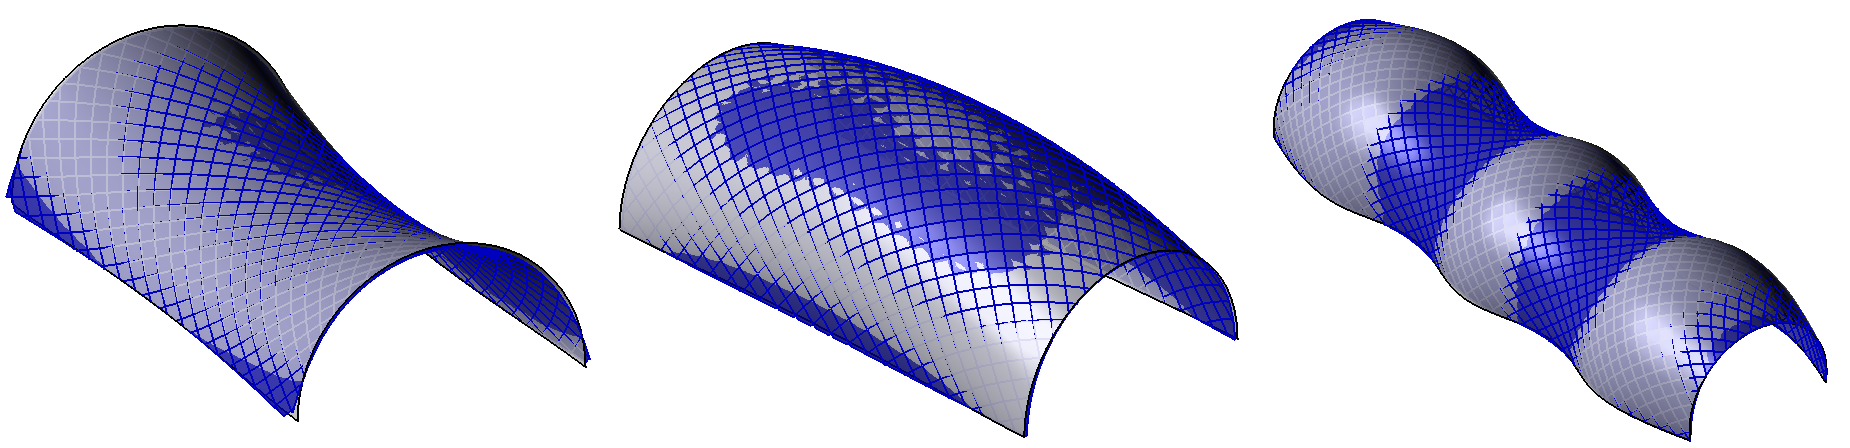
\includegraphics[width=1.0\linewidth]{images/CaseStudies_Regular/Compass_SurfaceComparison.png}
\caption{Deformation of the grids by allowing more distance from the reference surface}
\label{fig:Compass_SurfaceComparison}
\end{figure}

The anticlastic, synclastic and Downland-like gridshells have been further optimised by reducing the weighting factor of the {\it reference surface} energy and with it allowing a spacing between grid and target surface up to 0.6 m. Depending on the curvature distribution, the grids have been deformed above or below the reference surface.

On the case of the anticlastic gridshell, the corners of the lateral sides deform outside reducing here the maximum curvature values up to 45\% and obtaining a more homogeneous distribution on the centre of the gridshell. The mean curvature of the profiles could be reduced up to 51\%. By the synclastic gridshell, the lateral edges tend to distort outwards in the middle and the crown of the grid slightly upwards. The maximum and mean profiles curvatures were reduced up to 79\% and 78\%, respectively. By the gridshell with anticlastic and synclastic curvatures, the crowns deform inwards and the valleys outwards getting a flatter surface. The maximum and mean curvatures of the profiles could be reduced here up to 76\% and 64\%, respectively (see Fig.~\ref{fig:Compass_SurfaceComparison}).

\begin{figure}[t]
\centering
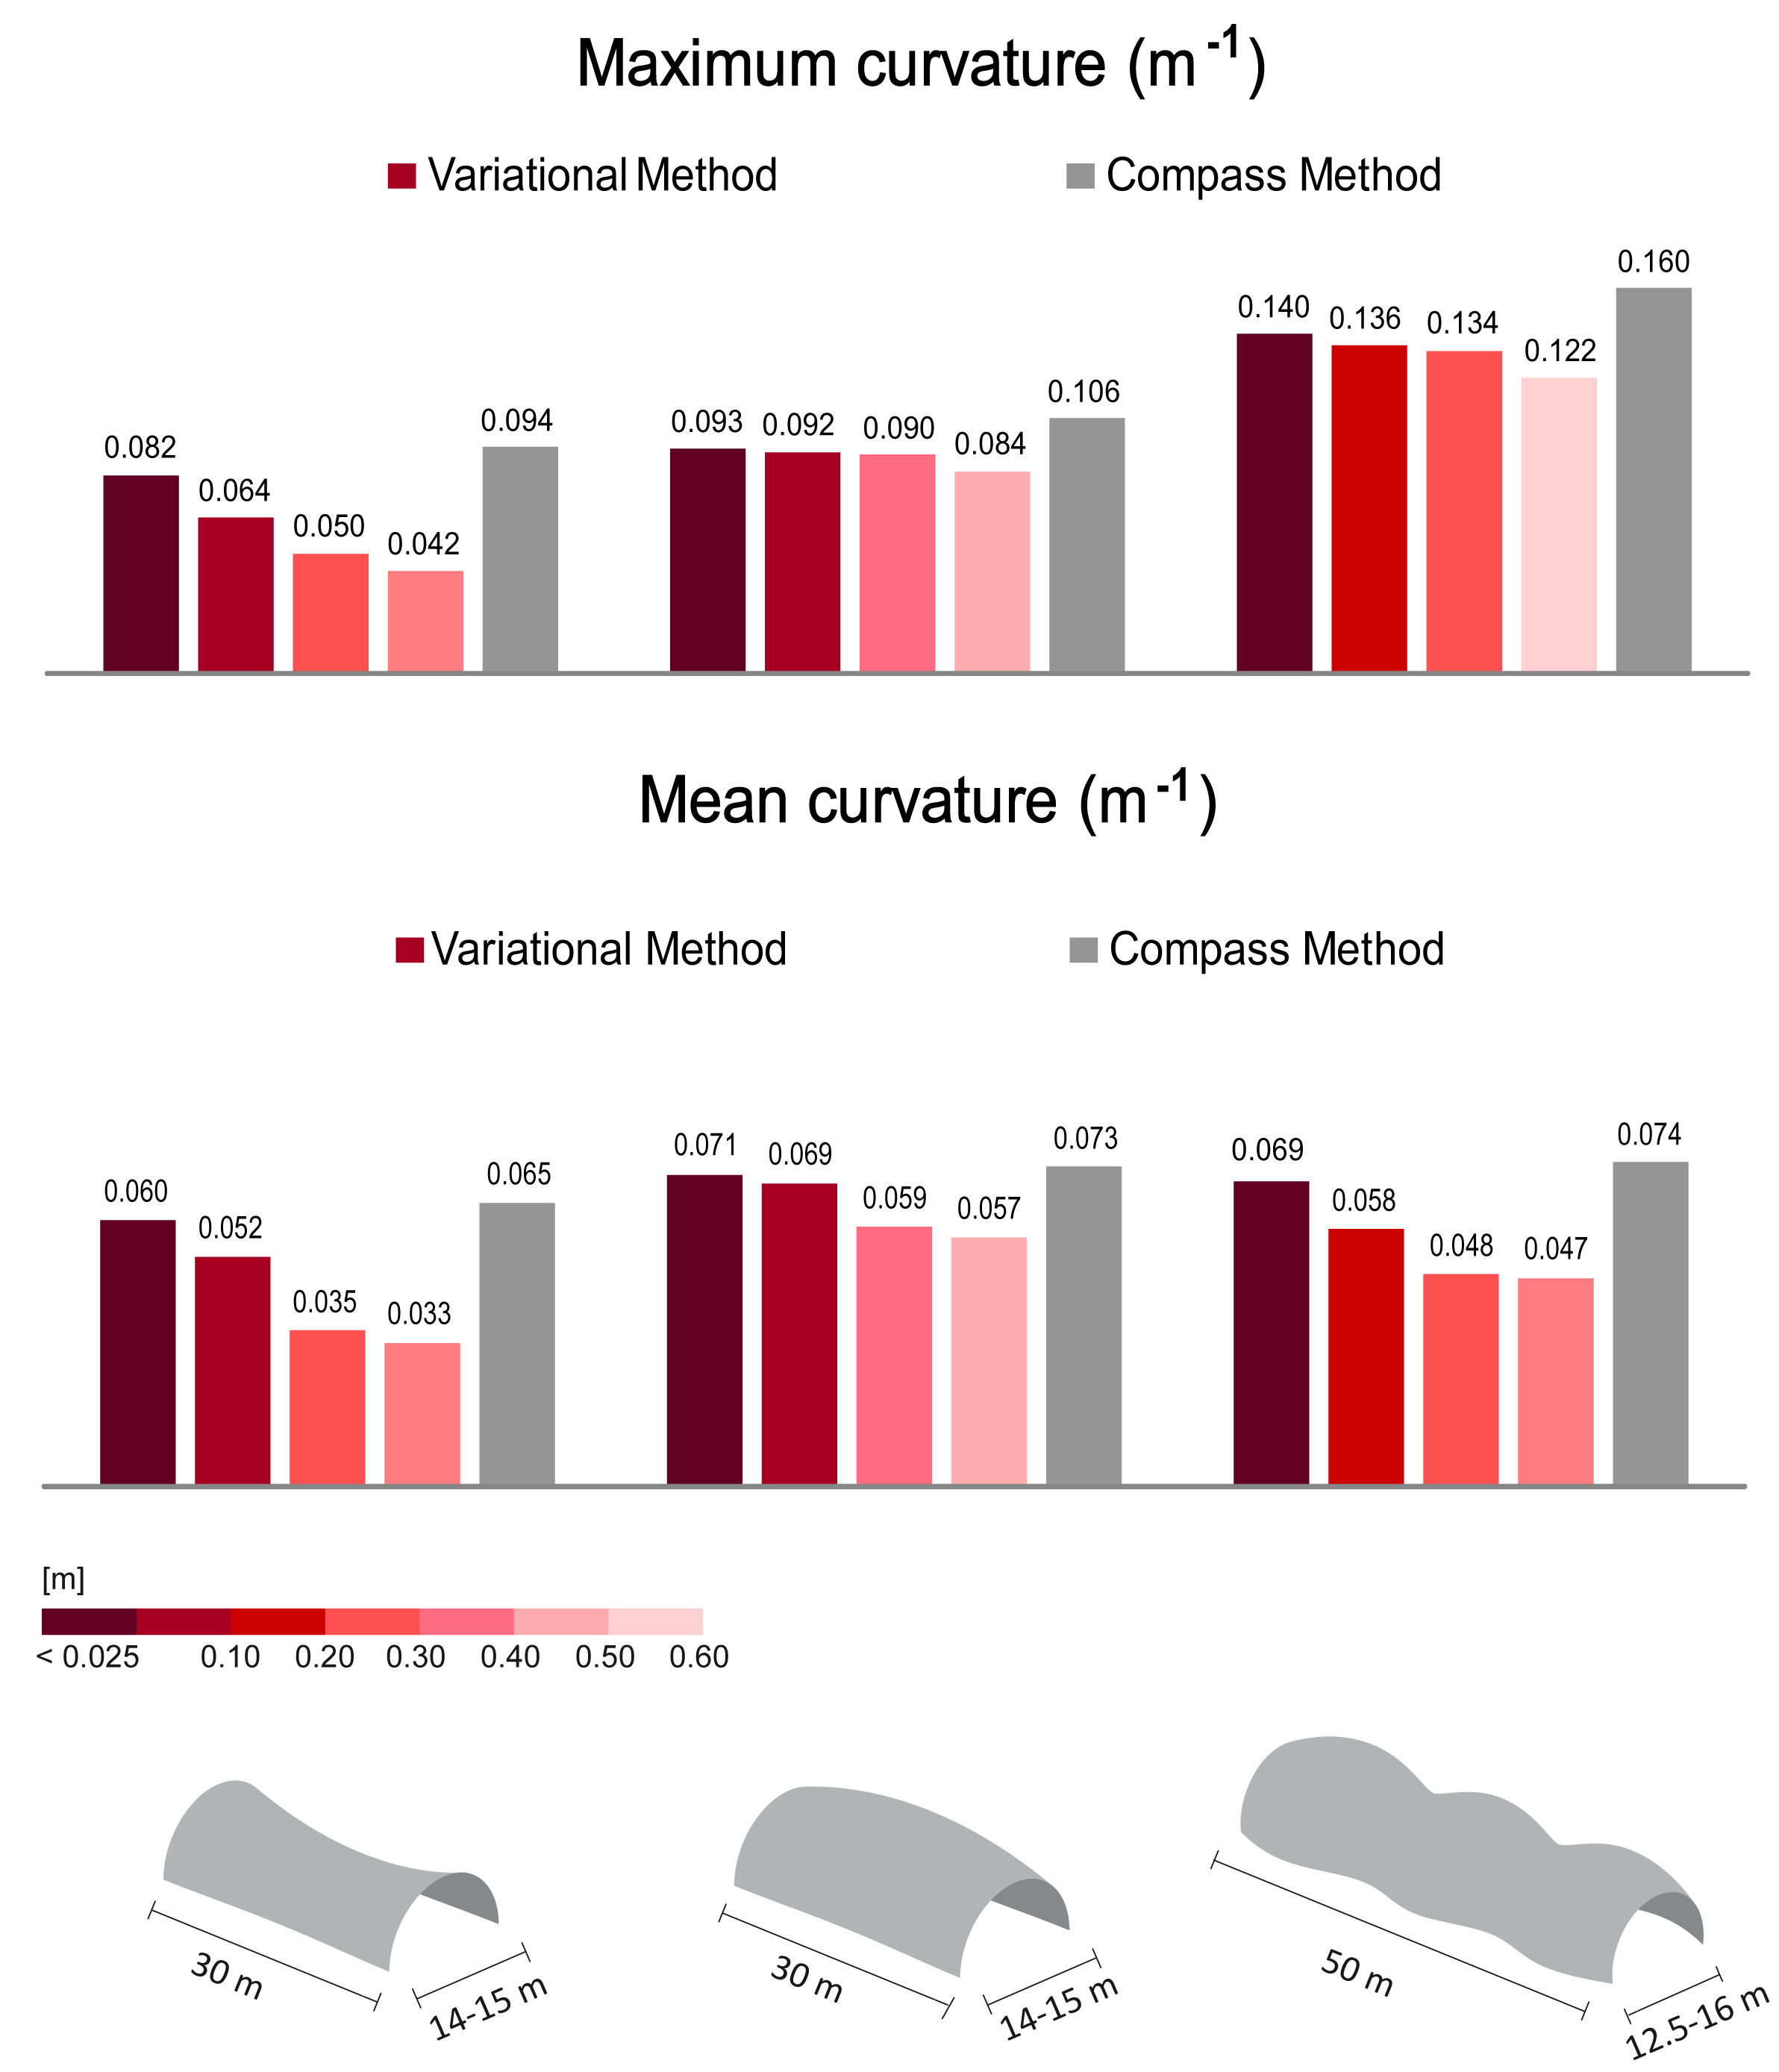
\includegraphics[width=0.80\linewidth]{images/CaseStudies_Regular/Balken.png}
\caption{Comparison of the maximum and mean profile curvatures of the anticlastic, synclastic and Downland-like grid topologies resulting from the variational and compass methods}
\label{fig:Balken}
\end{figure}

The following diagram  (Fig.~\ref{fig:Balken}) outlines the optimisation results achieved with the variational method in comparison to the compass method. The maximum and mean curvatures are illustrated for the three gridshells. The colour of the bars represents the distance from the reference surface. Generally, a higher reduction of the mean curvature is achieved, as the energy $E_{\textrm{\scriptsize{cur}}}$ to be minimised corresponds to the sum of all curvature values.





